\documentclass[10]{article}
%\documentclass[11pt]{book}
\usepackage{hyperref}
\usepackage{amsfonts,amssymb,amsmath,amsthm,cite}
\usepackage{graphicx}
\usepackage[toc,page]{appendix}
\usepackage{nicefrac}
%% \usepackage[francais]{babel}
\usepackage[applemac]{inputenc}
\usepackage{amssymb, euscript}
\usepackage[matrix,arrow,curve]{xy}
\usepackage{graphicx}
\usepackage{tabularx}
\usepackage{float}
\usepackage{tikz}
\usepackage{slashed}
\usepackage{mathrsfs}
\usepackage{multirow}

%\usepackage{mathtools}

\usetikzlibrary{matrix}

\usepackage[T1]{fontenc}
\usepackage{amsfonts,cite}
\usepackage{graphicx}

%% \usepackage[francais]{babel}
\usepackage[applemac]{inputenc}


\usepackage[sc]{mathpazo}
\usepackage{environ}

\linespread{1.05}         % Palatino needs more leading (space between lines)


%\usepackage[usenames]{color}



\DeclareFontFamily{T1}{pzc}{}
\DeclareFontShape{T1}{pzc}{m}{it}{1.8 <-> pzcmi8t}{}
\DeclareMathAlphabet{\mathpzc}{T1}{pzc}{m}{it}
% the command for it is \mathpzc

\textwidth=140mm


% % % % % % % % % % % % % % % % % % % %
\theoremstyle{plain}
\newtheorem{prop}{Proposition}[section]
\newtheorem{prdf}[prop]{Proposition and Definition}
\newtheorem{lem}[prop]{Lemma}%[section]
\newtheorem{cor}[prop]{Corollary}%[section]
\newtheorem{thm}[prop]{Theorem}%[section]
\newtheorem{theorem}[prop]{Theorem}
\newtheorem{lemma}[prop]{Lemma}
\newtheorem{proposition}[prop]{Proposition}
\newtheorem{corollary}[prop]{Corollary}
\newtheorem{statement}[prop]{Statement}

\theoremstyle{definition}
\newtheorem{defn}[prop]{Definition}%[section]
\newtheorem{cordefn}[prop]{Corollary and Definition}%[section]
\newtheorem{empt}[prop]{}%[section]
\newtheorem{exm}[prop]{Example}%[section]
\newtheorem{rem}[prop]{Remark}%[section]
\newtheorem{prob}[prop]{Problem}
\newtheorem{conj}{Conjecture}       %% Hypothesis 1
\newtheorem{cond}{Condition}        %% Condition 1
%\newtheorem{axiom}[thm]{Axiom}           %% Axiom 1 modified
\newtheorem{fact}[prop]{Fact}
\newtheorem{ques}{Question}         %% Question 1
\newtheorem{answ}{Answer}           %% Answer 1
\newtheorem{notn}{Notation}        %% Notations are not numbered

\theoremstyle{definition}
\newtheorem{notation}[prop]{Notation}
\newtheorem{definition}[prop]{Definition}
\newtheorem{example}[prop]{Example}
\newtheorem{exercise}[prop]{Exercise}
\newtheorem{conclusion}[prop]{Conclusion}
\newtheorem{conjecture}[prop]{Conjecture}
\newtheorem{criterion}[prop]{Criterion}
\newtheorem{summary}[prop]{Summary}
\newtheorem{axiom}[prop]{Axiom}
\newtheorem{problem}[prop]{Problem}
%\theoremstyle{remark}
\newtheorem{remark}[prop]{Remark}

\numberwithin{equation}{section}
\newtheorem*{claim}{Claim}
\DeclareMathOperator{\Dom}{Dom}              %% domain of an operator
\newcommand{\Dslash}{{D\mkern-11.5mu/\,}}    %% Dirac operator


%\newcommand\myeq{\stackrel{\mathclap{\normalfont\mbox{def}}}{=}}
\newcommand{\nor}[1]{\left\Vert #1\right\Vert}    %\nor{x}=||x||
\newcommand{\vertiii}[1]{{\left\vert\kern-0.25ex\left\vert\kern-0.25ex\left\vert #1
		\right\vert\kern-0.25ex\right\vert\kern-0.25ex\right\vert}}
\newcommand{\Ga}{\Gamma}  
\newcommand{\coker}{\mathrm{coker}}                   %% short for  \Gamma
\newcommand{\Coo}{C^\infty}                  %% smooth functions
% % % % % % % % % % % % % % % % % % % %


\usepackage[sc]{mathpazo}
\linespread{1.05}         % Palatino needs more leading (space between lines)

\newbox\ncintdbox \newbox\ncinttbox %% noncommutative integral symbols
\setbox0=\hbox{$-$} \setbox2=\hbox{$\displaystyle\int$}
\setbox\ncintdbox=\hbox{\rlap{\hbox
		to \wd2{\hskip-.125em \box2\relax\hfil}}\box0\kern.1em}
\setbox0=\hbox{$\vcenter{\hrule width 4pt}$}
\setbox2=\hbox{$\textstyle\int$} \setbox\ncinttbox=\hbox{\rlap{\hbox
		to \wd2{\hskip-.175em \box2\relax\hfil}}\box0\kern.1em}

\newcommand{\ncint}{\mathop{\mathchoice{\copy\ncintdbox}%
		{\copy\ncinttbox}{\copy\ncinttbox}%
		{\copy\ncinttbox}}\nolimits}  %% NC integral

%%% Repeated relations:
\newcommand{\xyx}{\times\cdots\times}      %% repeated product
\newcommand{\opyop}{\oplus\cdots\oplus}    %% repeated direct sum
\newcommand{\oxyox}{\otimes\cdots\otimes}  %% repeated tensor product
\newcommand{\wyw}{\wedge\cdots\wedge}      %% repeated exterior product
\newcommand{\subysub}{\subset\hdots\subset}      %% repeated subset
\newcommand{\supysup}{\supset\hdots\supset}      %% repeated supset
\newcommand{\rep}{\mathfrak{rep}}
\newcommand{\lift}{\mathfrak{lift}}
\newcommand{\desc}{\mathfrak{desc}}
%%% Roman letters:
\newcommand{\id}{\mathrm{id}}                %% identity map
\newcommand{\Id}{\mathrm{Id}}                %% identity map
\newcommand{\pt}{\mathrm{pt}}                %% a point
\newcommand{\const}{\mathrm{const}}          %% a constant
\newcommand{\codim}{\mathrm{codim}}          %% codimension
\newcommand{\cyc}{\mathrm{cyclic}}  %% cyclic sum
\renewcommand{\d}{\mathrm{d}}       %% commutative differential
\newcommand{\dR}{\mathrm{dR}}       %% de~Rham cohomology
\newcommand{\proj}{\mathrm{proj}}                %% a projection



\newcommand*{\Mult}{\mathcal M}% multiplier algebra

\newcommand{\A}{\mathcal{A}}                 %%\newcommand{\unitsv}[1]{#1^{(0)}}
\newcommand{\units}{G^{(0)}}
\newcommand{\haars}{\{\lambda^{u}\}_{u\in\units}}
\newcommand{\shaars}{\{\lambda_{u}\}_{u\in\units}}
\newcommand{\haarsv}[2]{\{\lambda^{#2}_{#1}\}_{#2\in\unitsv{#1}}}
\newcommand{\haarv}[2]{\lambda^{#2}_{#1}}

\renewcommand{\a}{\alpha}                    %% short for  \alphapha
\DeclareMathOperator{\ad}{ad}                %% infml adjoint repn
\newcommand{\as}{\quad\mbox{as}\enspace}     %% `as' with spacing
\newcommand{\Aun}{\widetilde{\mathcal{A}}}   %% unital algebra
\newcommand{\B}{\mathcal{B}}                 %% space of distributions
\newcommand{\E}{\mathcal{E}}                 %% space of distributions
\renewcommand{\b}{\beta}                     %% short for \beta
\newcommand{\braCket}[3]{\langle#1\mathbin|#2\mathbin|#3\rangle}
\newcommand{\braket}[2]{\langle#1\mathbin|#2\rangle} %% <w|z>
\newcommand{\C}{\mathbb{C}}                  %% complex numbers
\newcommand{\CC}{\mathcal{C}}                %% space of distributions
\newcommand{\cc}{\mathbf{c}}                 %% Hochschild cycle
\DeclareMathOperator{\Cl}{C\ell}             %% Clifford algebra
\newcommand{\F}{\mathcal{F}}                 %% space of test functions
\newcommand{\G}{\mathcal{G}}                 %% 
\newcommand{\D}{\mathcal{D}}                 %% Moyal L^2-filtration
\renewcommand{\H}{\mathcal{H}}               %% Hilbert space
\newcommand{\half}{\tfrac{1}{2}}             %% small fraction  1/2
\newcommand{\hh}{\mathcal{H}}                %% Hilbert space
\newcommand{\hookto}{\hookrightarrow}        %% abbreviation
\newcommand{\Ht}{{\widetilde{\mathcal{H}}}}  %% Hilbert space of forms
\newcommand{\I}{\mathcal{I}}                 %% tracelike functions
\DeclareMathOperator{\Junk}{Junk}            %% the junk DGA ideal
\newcommand{\K}{\mathcal{K}}                 %% compact operators
\newcommand{\ket}[1]{|#1\rangle}             %% ket vector
\newcommand{\ketbra}[2]{|#1\rangle\langle#2|} %% rank one operator
\renewcommand{\L}{\mathcal{L}}               %% operator algebra
\newcommand{\La}{\Lambda}                    %% short for \Lambda
\newcommand{\la}{\lambda}                    %% short for \lambda
\newcommand{\lf}{L_f^\theta}                 %% left mult operator
\newcommand{\M}{\mathcal{M}}                 %% Moyal multplr algebra
\newcommand{\mm}{\mathcal{M}^\theta}
%\newcommand{{{\star_{\theta}}}{{\mathchoice{\mathbin{\;|\;ar_{_\theta}}}
			%            {\mathbin{\;|\;ar_{_\theta}}}           %% Moyal
			%            {{\;|\;ar_\theta}}{{\;|\;ar_\theta}}}}    %% product
	\newcommand{\N}{\mathbb{N}}                  %% nonnegative integers
	\newcommand{\NN}{\mathcal{N}}                %% a Moyal algebra
	\newcommand{\nb}{\nabla}                     %% gradient
	\newcommand{\Oh}{\mathcal{O}}                %% comm multiplier alg
	\newcommand{\om}{\omega}                     %% short for \omega
	\newcommand{\opp}{{\mathrm{op}}}             %% opposite algebra
	\newcommand{\ox}{\otimes}                    %% tensor product
	\newcommand{\eps}{\varepsilon}                    %% tensor product
	\newcommand{\otimesyox}{\otimes\cdots\otimes}    %% repeated tensor product
	\newcommand{\pa}{\partial}                   %% short for \partial
	\newcommand{\pd}[2]{\frac{\partial#1}{\partial#2}}%% partial derivative
	\newcommand{\piso}[1]{\lfloor#1\rfloor}      %% integer part
	\newcommand{\PsiDO}{\Psi~\mathrm{DO}}         %% pseudodiffl operators
	\newcommand{\Q}{\mathbb{Q}}                  %% rational numbers
	\newcommand{\R}{\mathbb{R}}                  %% real numbers
	\newcommand{\rdl}{R_\Dslash(\lambda)}        %% resolvent
	\newcommand{\roundbraket}[2]{(#1\mathbin|#2)} %% (w|z)
	\newcommand{\row}[3]{{#1}_{#2},\dots,{#1}_{#3}} %% list: a_1,...,a_n
	\newcommand{\sepword}[1]{\quad\mbox{#1}\quad} %% well-spaced words
	\newcommand{\set}[1]{\{\,#1\,\}}             %% set notation
	\newcommand{\Sf}{\mathbb{S}}                 %% sphere
	\newcommand{\uhor}[1]{\Omega^1_{hor}#1}
	\newcommand{\sco}[1]{{\sp{(#1)}}}
	\newcommand{\sw}[1]{{\sb{(#1)}}}
	\DeclareMathOperator{\spec}{sp}              %% spectrum
	\renewcommand{\SS}{\mathcal{S}}              %% Schwartz space
	\newcommand{\sss}{\mathcal{S}}               %% Schwartz space
	\DeclareMathOperator{\supp}{\mathfrak{supp}}            %% support
	\newcommand{\T}{\mathbb{T}}                  %% circle as a group
	\renewcommand{\th}{\theta}                   %% short for \theta
	\newcommand{\thalf}{\tfrac{1}{2}}            %% small* fraction 1/2
	\newcommand{\tihalf}{\tfrac{i}{2}}           %% small* fraction i/2
	\newcommand{\tpi}{{\tilde\pi}}               %% extended representation
	\DeclareMathOperator{\Tr}{Tr}                %% trace of operator
	\DeclareMathOperator{\tr}{tr}                %% trace of matrix
	\newcommand{\del}{\partial}                  %% short for  \partial
	\DeclareMathOperator{\tsum}{{\textstyle\sum}} %% small sum in display
	\newcommand{\V}{\mathcal{V}}                 %% test function space
	\newcommand{\vac}{\ket{0}}                   %% vacuum ket vector
	\newcommand{\vf}{\varphi}                    %% scalar field
	\newcommand{\w}{\wedge}                      %% exterior product
	\DeclareMathOperator{\wres}{wres}            %% density of Wresidue
	\newcommand{\x}{\times}                      %% cross
	\newcommand{\Z}{\mathbb{Z}}                  %% integers
	\newcommand{\7}{\dagger}                     %% short for + symbol
	\newcommand{\8}{\bullet}                     %% anonymous degree
	\renewcommand{\.}{\cdot}                     %% anonymous variable
	\renewcommand{\:}{\colon}                    %% colon in  f: A -> B
	
	%\newcommand{\sA}{\mathscr{A}}       %%
	\newcommand{\sA}{\mathcal{A}} 
	\newcommand{\sB}{\mathcal{B}}       %%
	\newcommand{\sC}{\mathcal{C}}       %%
	\newcommand{\sD}{\mathcal{D}}       %%
	\newcommand{\sE}{\mathcal{E}}       %%
	\newcommand{\sF}{\mathcal{F}}       %%
	\newcommand{\sG}{\mathcal{G}}       %%
	\newcommand{\sH}{\mathcal{H}}       %%
	\newcommand{\sI}{\mathcal{I}}       %%
	\newcommand{\sJ}{\mathcal{J}}       %%
	\newcommand{\sK}{\mathcal{K}}       %%
	\newcommand{\sL}{\mathcal{L}}       %%
	\newcommand{\sM}{\mathcal{M}}       %%
	\newcommand{\sN}{\mathcal{N}}       %%
	\newcommand{\sO}{\mathcal{O}}       %%
	\newcommand{\sP}{\mathcal{P}}       %%
	\newcommand{\sQ}{\mathcal{Q}}       %%
	\newcommand{\sR}{\mathcal{R}}       %%
	\newcommand{\sS}{\mathcal{S}}       %%
	\newcommand{\sT}{\mathcal{T}}       %%
	\newcommand{\sU}{\mathcal{U}}       %%
	\newcommand{\sV}{\mathcal{V}}       %%
	\newcommand{\sX}{\mathcal{X}}       %%
	\newcommand{\sY}{\mathcal{Y}}       %%
	\newcommand{\sZ}{\mathcal{Z}}       %%
	
	\newcommand{\Om}{\Omega}       %%
	
	
	\DeclareMathOperator{\ptr}{ptr}     %% Poisson trace
	\DeclareMathOperator{\Trw}{Tr_\omega} %% Dixmier trace
	\DeclareMathOperator{\vol}{Vol}     %% total volume
	\DeclareMathOperator{\Vol}{Vol}     %% total volume
	\DeclareMathOperator{\Area}{Area}   %% area of a surface
	\DeclareMathOperator{\Wres}{Wres}   %% (Wodzicki) residue
	
	\newcommand{\dd}[1]{\frac{\partial}{\partial#1}}   %% partial derivation
	\newcommand{\ddt}[1]{\frac{d}{d#1}}                %% derivative
	\newcommand{\inv}[1]{\frac{1}{#1}}                 %% inverse
	\newcommand{\sfrac}[2]{{\scriptstyle\frac{#1}{#2}}} %% tiny fraction
	
	\newcommand{\bA}{\mathbb{A}}       %%
	\newcommand{\bB}{\mathbb{B}}       %%
	\newcommand{\bC}{\mathbb{C}}       %%
	\newcommand{\bCP}{\mathbb{C}P}     %%
	\newcommand{\bD}{\mathbb{D}}       %%
	\newcommand{\bE}{\mathbb{E}}       %%
	\newcommand{\bF}{\mathbb{F}}       %%
	\newcommand{\bG}{\mathbb{G}}       %%
	\newcommand{\bH}{\mathbb{H}}       %%
	\newcommand{\bHP}{\mathbb{H}P}     %%
	\newcommand{\bI}{\mathbb{I}}       %%
	\newcommand{\bJ}{\mathbb{J}}       %%
	\newcommand{\bK}{\mathbb{K}}       %%
	\newcommand{\bL}{\mathbb{L}}       %%
	\newcommand{\bM}{\mathbb{M}}       %%
	\newcommand{\bN}{\mathbb{N}}       %%
	\newcommand{\bO}{\mathbb{O}}       %%
	\newcommand{\bOP}{\mathbb{O}P}     %%
	\newcommand{\bP}{\mathbb{P}}       %%
	\newcommand{\bQ}{\mathbb{Q}}       %%
	\newcommand{\bR}{\mathbb{R}}       %%
	\newcommand{\bRP}{\mathbb{R}P}     %%
	\newcommand{\bS}{\mathbb{S}}       %%
	\newcommand{\bT}{\mathbb{T}}       %%
	\newcommand{\bU}{\mathbb{U}}       %%
	\newcommand{\bV}{\mathbb{V}}       %%
	\newcommand{\bX}{\mathbb{X}}       %%
	\newcommand{\bY}{\mathbb{Y}}       %%
	\newcommand{\bZ}{\mathbb{Z}}       %%
	
	\newcommand{\bydef}{\stackrel{\mathrm{def}}{=}}          %% 
	
	
	\newcommand{\al}{\alpha}          %% short for  \alpha
	\newcommand{\bt}{\beta}           %% short for  \beta
	\newcommand{\Dl}{\Delta}          %% short for  \Delta
	\newcommand{\dl}{\delta}          %% short for  \delta
	\newcommand{\ga}{\gamma}          %% short for  \gamma
	\newcommand{\ka}{\kappa}          %% short for  \kappa
	\newcommand{\sg}{\sigma}          %% short for  \sigma
	\newcommand{\Sg}{\Sigma}          %% short for  \Sigma
	\newcommand{\Th}{\Theta}          %% short for  \Theta
	\renewcommand{\th}{\theta}        %% short for  \theta
	\newcommand{\vth}{\vartheta}      %% short for  \vartheta
	\newcommand{\ze}{\zeta}           %% short for  \zeta
	
	\DeclareMathOperator{\ord}{ord}     %% order of a PsiDO
	\DeclareMathOperator{\rank}{rank}   %% rank of a vector bundle
	\DeclareMathOperator{\sign}{sign}   %%
	\DeclareMathOperator{\sgn}{sgn}   %%
	\DeclareMathOperator{\chr}{char}   %%
	\DeclareMathOperator{\ev}{ev}       %% evaluation
	
	
	\newcommand{\Op}{\mathbf{Op}}
	\newcommand{\As}{\mathbf{As}}
	\newcommand{\Com}{\mathbf{Com}}
	\newcommand{\LLie}{\mathbf{Lie}}
	\newcommand{\Leib}{\mathbf{Leib}}
	\newcommand{\Zinb}{\mathbf{Zinb}}
	\newcommand{\Poiss}{\mathbf{Poiss}}
	
	\newcommand{\gX}{\mathfrak{X}}      %% vector fields
	\newcommand{\sol}{\mathfrak{so}}    %% special orthogonal Lie algebra
	\newcommand{\gm}{\mathfrak{m}}      %% maximal ideal
	
	
	\DeclareMathOperator{\Res}{Res}
	\DeclareMathOperator{\NCRes}{NCRes}
	\DeclareMathOperator{\Ind}{Ind}
	%% co/homology theories
	\DeclareMathOperator{\rH}{H}        %% any co/homology
	\DeclareMathOperator{\rC}{C}        %%  any co/chains
	\DeclareMathOperator{\rZ}{Z}        %% cycles
	\DeclareMathOperator{\rB}{B}        %% boundaries
	\DeclareMathOperator{\rF}{F}        %% filtration
	\DeclareMathOperator{\Gr}{gr}        %% associated graded object
	\DeclareMathOperator{\rHc}{H_{\mathrm{c}}}   %% co/homology with compact support
	\DeclareMathOperator{\drH}{H_{\mathrm{dR}}}  %% de Rham co/homology
	\DeclareMathOperator{\cechH}{\check{H}}    %% Cech co/homology
	\DeclareMathOperator{\rK}{K}        %% K-groups
	\DeclareMathOperator{\rKO}{KO}        %% real K-groups
	\DeclareMathOperator{\rKU}{KU}        %% unitary K-groups
	\DeclareMathOperator{\rKSp}{KSp}        %% symplectic K-groups
	\DeclareMathOperator{\rR}{R}        %% representation ring
	\DeclareMathOperator{\rI}{I}        %% augmentation ideal
	\DeclareMathOperator{\HH}{HH}       %% Hochschild co/homology
	\DeclareMathOperator{\HC}{HC}       %% cyclic co/homology
	\DeclareMathOperator{\HP}{HP}       %% periodic cyclic co/homology
	\DeclareMathOperator{\HN}{HN}       %% negative cyclic co/homology
	\DeclareMathOperator{\HL}{HL}       %% Leibniz co/homology
	\DeclareMathOperator{\KK}{KK}       %% KK-theory
	\DeclareMathOperator{\KKK}{\mathbf{KK}}       %% KK-theory as a category
	\DeclareMathOperator{\Ell}{Ell}       %% Abstract elliptic operators
	\DeclareMathOperator{\cd}{cd}       %% cohomological dimension
	\DeclareMathOperator{\spn}{span}       %% span
	\DeclareMathOperator{\linspan}{span} %% linear span (can't use \span)
	\newcommand{\blank}{-}   
	
	
	
	\newcommand{\twobytwo}[4]{\begin{pmatrix} #1 & #2 \\ #3 & #4 \end{pmatrix}}
	\newcommand{\CGq}[6]{C_q\!\begin{pmatrix}#1&#2&#3\\#4&#5&#6\end{pmatrix}}
	%% q-Clebsch--Gordan coefficients
	\newcommand{\cz}{{\bullet}}         %% anonymous degree
	\newcommand{\nic}{{\vphantom{\dagger}}} %% invisible dagger
	\newcommand{\ep}{{\dagger}}         %% abbreviation for + symbol
	\newcommand{\downto}{\downarrow}    %% right hand limit
	\newcommand{\isom}{\cong}          %% isomorphism
	\newcommand{\lt}{\triangleright}    %% a left action
	\newcommand{\otto}{\leftrightarrow} %% bijection
	\newcommand{\rt}{\triangleleft}     %% a right action
	\newcommand{\semi}{\rtimes}         %% crossed product
	\newcommand{\tensor}{\otimes}       %% tensor product
	\newcommand{\cotensor}{\square}       %% cotensor product
	\newcommand{\trans}{\pitchfork}     %% transverse
	\newcommand{\ul}{\underline}        %% for sheaves
	\newcommand{\upto}{\uparrow}        %% left hand limit
	\renewcommand{\:}{\colon}           %% colon in  f: A -> B
	\newcommand{\blt}{\ast}
	\newcommand{\Co}{C_{\bullet}}
	\newcommand{\cCo}{C^{\bullet}}
	\newcommand{\nbs}{\nabla^S}         %% spin connection
	\newcommand{\up}{{\mathord{\uparrow}}} %% `up' spinors
	\newcommand{\dn}{{\mathord{\downarrow}}} %% `down' spinors
	\newcommand{\updn}{{\mathord{\updownarrow}}} %% up or down
	
	%%% Bilinear enclosures:
	
	\newcommand{\bbraket}[2]{\langle\!\langle#1\stroke#2\rangle\!\rangle}
	%% <<w|z>>
	\newcommand{\bracket}[2]{\langle#1,\, #2\rangle} %% <w,z>
	\newcommand{\scalar}[2]{\langle#1,\,#2\rangle} %% <w,z>
	\newcommand{\poiss}[2]{\{#1,\,#2\}} %% {w,z}
	\newcommand{\dst}[2]{\langle#1,#2\rangle} %% distributions <u,\phi>
	\newcommand{\pairing}[2]{(#1\stroke #2)} %% right-linear pairing
	\def\<#1|#2>{\langle#1\stroke#2\rangle} %% \braket (Dirac notation)
	\def\?#1|#2?{\{#1\stroke#2\}}        %% left-linear pairing
	
	%%% Accent-like macros:
	
	\renewcommand{\Bar}[1]{\overline{#1}} %% closure operator
	\renewcommand{\Hat}[1]{\widehat{#1}}  %% short for \widehat
	\renewcommand{\Tilde}[1]{\widetilde{#1}} %% short for \widetilde
	
	
	\DeclareMathOperator{\bCl}{\bC l}   %% complex Clifford algebra
	
	%%% Small fractions in displays:
	
	\newcommand{\ihalf}{\tfrac{i}{2}}   %% small fraction  i/2
	\newcommand{\quarter}{\tfrac{1}{4}} %% small fraction  1/4
	\newcommand{\shalf}{{\scriptstyle\frac{1}{2}}}  %% tiny fraction  1/2
	\newcommand{\third}{\tfrac{1}{3}}   %% small fraction  1/3
	\newcommand{\ssesq}{{\scriptstyle\frac{3}{2}}} %% tiny fraction  3/2
	\newcommand{\sesq}{{\mathchoice{\tsesq}{\tsesq}{\ssesq}{\ssesq}}} %% 3/2
	\newcommand{\tsesq}{\tfrac{3}{2}}   %% small fraction  3/2
	
	
	%\newcommand\eqdef{\overset{\mathclap{\normalfont\mbox{def}}}{=}}
	\newcommand\eqdef{\overset{\mathrm{def}}{=}}
	
	
	%+++++++++++++++++++++++++++++++++++
	
	\newcommand{\word}[1]{\quad\text{#1}\enspace} %% well-spaced words
	\newcommand{\words}[1]{\quad\text{#1}\quad} %% better-spaced words
	\newcommand{\su}[1]{{\sp{[#1]}}}
	
	\def\<#1,#2>{\langle#1,#2\rangle}            %% bilinear pairing
	\def\ee_#1{e_{{\scriptscriptstyle#1}}}       %% basis projector
	\def\wick:#1:{\mathopen:#1\mathclose:}       %% Wick-ordered operator
	
	\newcommand{\opname}[1]{\mathop{\mathrm{#1}}\nolimits}
	
	\newcommand{\hideqed}{\renewcommand{\qed}{}} %% to suppress `\qed'
	
	
	%%%%%%%%%%%%%%%%%%%%%%%%%%%%%
	%% 2. Some internal machinery
	%%%%%%%%%%%%%%%%%%%%%%%%%%%%%
	
	\newbox\ncintdbox \newbox\ncinttbox %% noncommutative integral symbols
	\setbox0=\hbox{$-$}
	\setbox2=\hbox{$\displaystyle\int$}
	\setbox\ncintdbox=\hbox{\rlap{\hbox
			to \wd2{\box2\relax\hfil}}\box0\kern.1em}
	\setbox0=\hbox{$\vcenter{\hrule width 4pt}$}
	\setbox2=\hbox{$\textstyle\int$}
	\setbox\ncinttbox=\hbox{\rlap{\hbox
			to \wd2{\hskip-.05em\box2\relax\hfil}}\box0\kern.1em}
	
	\newcommand{\disp}{\displaystyle} %% short for  \displaystyle
	
	%\newcommand{\hideqed}{\renewcommand{\qed}{}} %% no `\qed' at end-proof
	
	\newcommand{\stroke}{\mathbin|}   %% (for `\bbraket' and such)
	\newcommand{\tribar}{|\mkern-2mu|\mkern-2mu|} %% norm bars: |||
	
	%%% Enclose one argument with delimiters:
	
	\newcommand{\bra}[1]{\langle{#1}\rvert} %% bra vector <w|
	\newcommand{\kett}[1]{\lvert#1\rangle\!\rangle} %% ket 2-vector |y>>
	\newcommand{\snorm}[1]{\mathopen{\tribar}{#1}%
		\mathclose{\tribar}}                 %% norm |||x|||
	
	
	\newcommand{\End}{\mathrm{End}}       %%
	\newcommand{\Ext}{\mathrm{Ext}}       %%
	\newcommand{\Hom}{\mathrm{Hom}}       %%
	\newcommand{\Mrt}{\mathrm{Mrt}}       %%
	\newcommand{\grad}{\mathrm{grad}}       %%
	\newcommand{\Spin}{\mathrm{Spin}}       %%
	\newcommand{\Ad}{\mathrm{Ad}}       %%
	\newcommand{\Pic}{\mathrm{Pic}}       %%
	\newcommand{\Aut}{\mathrm{Aut}}       %%
	\newcommand{\Inn}{\mathrm{Inn}}       %%
	\newcommand{\Out}{\mathrm{Out}}       %%
	\newcommand{\Homeo}{\mathrm{Homeo}}       %%
	\newcommand{\Diff}{\mathrm{Diff}}       %%
	\newcommand{\im}{\mathrm{im}}       %%
	
	
	\newcommand{\SO}{\mathrm{SO}}       %%
	\newcommand{\SU}{SU}       %%
	\newcommand{\gso}{\mathfrak{so}}    %% special orthogonal Lie algebra
	\newcommand{\gero}{\mathfrak{o}}    %% orthogonal Lie algebra
	\newcommand{\gspin}{\mathfrak{spin}} %% spin Lie algebra
	\newcommand{\gu}{\mathfrak{u}}      %% unitary Lie algebra
	\newcommand{\gsu}{\mathfrak{su}}    %% special unitary Lie algebra
	\newcommand{\gsl}{\mathfrak{sl}}    %% special linear Lie algebra
	\newcommand{\gsp}{\mathfrak{sp}}    %% symplectic linear Lie algebra
	
	%\newcommand{\bes}{\begin{equation}\begin{split}}
			%\newcommand{\ees}{\end{split}\end{equation}}
	%\NewEnviron{split.enviro}{%
		%	\begin{equation}\begin{split}
				%	\BODY
				%	\end{split}\end{equation}
		%$}
	\newenvironment{splitequation}{\begin{equation}\begin{split}}{\end{split}\end{equation}}
	
	%Begin equation split: Begin equation split = bes
	\newcommand{\bs}{\begin{split}}
		\newcommand{\es}{\end{split}}
	\newcommand{\be}{\begin{equation}}
		\renewcommand{\ee}{\end{equation}}
	\newcommand{\bea}{\begin{eqnarray}}
		\newcommand{\eea}{\end{eqnarray}}
	\newcommand{\bean}{\begin{eqnarray*}}
		\newcommand{\eean}{\end{eqnarray*}}
	\newcommand{\brray}{\begin{array}}
		\newcommand{\erray}{\end{array}}
	\newenvironment{equations}
	{\begin{equation}
			\begin{split}}
			{\end{split}
	\end{equation}}
	\newcommand{\Hsquare}{%
		\text{\fboxsep=-.2pt\fbox{\rule{0pt}{1ex}\rule{1ex}{0pt}}}%
	}
	
	\title{Grothendieck topology of  $C^*$-algebras}
	
	\author
	{\textbf{Petr R. Ivankov*}\\
		e-mail: * monster.ivankov@gmail.com \\
	}
	
	\begin{document}

\maketitle  %\setlength{\parindent}{0pt}
\pagestyle{plain}


%\vspace{1 in}


%\noindent

\begin{abstract}
For any topological space there is a sheaf cohomology. A Grothendieck topology  is a generalization  of the  classical topology such that  it also possesses a sheaf cohomology. On the other hand any noncommutative $C^*$-algebra is a generalization of a locally compact Hausdorff space. Here we define a Grothendieck topology arising from  $C^*$-algebras which is a generalization of the topology of the spectra of commutative $C^*$-algebras. This construction yields a noncommutative generalization of the sheaf cohomology of topological spaces.  If $A$ is a $C^*$-algebra of type $I_0$ then its Grothendieck topology can be represented by a topological space. There is an analogy between the Dixmier-Douady theory  of continuous-trace $C^*$-algebras and Grothendieck topology of $C^*$-algebras of type $I_0$.
\end{abstract}


%\end{abstract}

\section{General theory}
\paragraph*{}

	If $A$ is a $C^*$-algebra then there is a category $\mathbf{Hered}/A$ such that:
\begin{itemize}
	\item $\mathbf{Hered}/A$-objects are hereditary $C^*$- subalgebras of $A$,
	\item $\mathbf{Hered}/A$-morphism  from $B' \subset A$ to $B'' \subset A$ is a natural inclusion $B'\subset B''$ such that a following diagram 
	\newline
	\begin{tikzpicture}
		\matrix (m) [matrix of math nodes,row sep=3em,column sep=4em,minimum width=2em]
		{
			B'  &  & B''\\ 
			& A &\\};
		\path[-stealth]
		(m-1-1) edge node [above] {$\subset$} (m-1-3)
		(m-1-1) edge node [above]  {} (m-2-2)
		(m-1-3) edge node [right]  {} (m-2-2);
	\end{tikzpicture}
	\\
	is commutative.
\end{itemize}
For any two $\mathbf{Hered}/A$-objects $B', B''$ we define their \textit{fibre product} (cf. Definition \ref{pullback_defn}) by the following way
$$
B'\times_A B'' \bydef B'\cap B''.
$$

\begin{definition}\label{hered_cov_defn}
For any $\mathbf{Hered}/A$-object $B$ a distinguished set of families of inclusions $\left\{B_\iota \subset B\right\}_{\iota\in I}$, called a \textit{covering} of $B$ if $B$ is a generated by the union $\cup B_\iota$ hereditary $C^*$-subalgebra of $A$ (cf. Definition \ref{hered_generated_defn}).
\end{definition}

\begin{lemma}\label{grothendieck_ca_lem}
A given by the Definition \ref{hered_cov_defn} system of coverings satisfies to  the Definition \ref{site_defn}, so one has a natural Grothendieck topology.
\end{lemma}
\begin{proof}
	If $A$ be a $C^*$-algebra, then one needs check that hereditary $C^*$-subalgebras of $A$ satisfy to axioms (a)-(c) of the Definition \ref{site_defn}.\\
	(a) Let $B, C\subset A$ be subalgebras. A covering of $B$ is a family $\left\{B_\iota\subset B\right\}_{\iota \in I}$ of subalgebras of $B$ such that $B$ is a generated by a union $\bigcup B_\iota$ hereditary $C^*$-subalgebra (cf. Definition \ref{hered_generated_defn}). If  $L\left( B\right)$, $L\left( C\right)$ and $L\left( B_\iota \right)$ are given by the equation \eqref{left_ideal_eqn} closed left ideals then $L\left(B\cap C \right) = L(B)\cap L(C)$, $~L\left(B_\iota \cap C \right)= L\left(B_\iota \right)\cap L\left( C \right)$ (cf. Lemma \ref{hered_ideal_lem}). Moreover $L\left(B\right)$ is the $C^*$-norm closure of an algebraic sum $\sum_{\iota\in I} L\left( B_\iota\right)$. For any $\iota \in I$ one has $L\left(B_\iota\right)\cap L\left(C\right)\subset L\left(B\right)\cap L\left(C\right)$ it follows that $\sum_{\iota\in I} \left( L\left(B_\iota\right)\cap L\left(C\right)\right) \subset L\left(B\right)\cap L\left(C\right)$. Since the left ideal  $L\left(B\right)\cap L\left(C\right)$ is $C^*$-norm closed the $C^*$-norm closure of an algebraic sum $\sum_{\iota\in I} \left( L\left(B_\iota\right)\cap L\left(C\right)\right)$ is a subset of  the intersection $L\left(B\right)\cap L\left(C\right)$ i.e. a generated by a union $\cup_\iota \left( B_\iota\cup C\right)$ hereditary subalgebra is a subalgebra of the intersection $B\cap C$. If $\eps > 0$ and $ b\in L\left(C\right)\cap L\left(B\right)$ then from the from the Theorem \ref{left_ideal_thm} it follows that there is a positive $u \in L\left(C\right)$ such that 
	\bean
	\left\|u \right\| \le 1,\\
	\left\|b - b u\right\|< \frac{\eps}{2}.
	\eean 
	Since the set $\sum_{\iota\in I}  L\left(B_\iota\right)$ is dense in $L\left(B\right)$ there is a sum $\sum_{k = 1}^n b_{k}$ such that
	\bean
	\forall k\in \{1,..., n\}\quad \exists \iota_k\in I \quad b_k \in L\left( B_{\iota_k}\right)  ,\\
		\left\|b - \sum_{k = 1}^n b_k \right\|< \frac{\eps}{2}.
		\eean
		Applying the triangle identity one has
	$$
	\left\|b -  \left( \sum_{k = 1}^n b_k\right)  u\right\|	\le 	\left\|\left( b -   \sum_{k = 1}^n b_k\right)  u\right\|+ \left\|b -   b  u\right\|< \left\| b -   \sum_{k = 1}^n b_k\right\|\left\|  u\right\|+ \frac{\eps}{2}< \eps.
$$
From the following circumstances:
\begin{itemize}
	\item  the number $\eps$ is arbitrary small,
	\item $\left( \sum_{k = 1}^n b_k\right)  u\in \sum_{\iota\in I} \left( L\left(B_\iota\right)\cap L\left(C\right)\right)$
\end{itemize}
we conclude that $b$ lies in the $C^*$-norm closure of $\sum_{\iota\in I} \left( L\left(B_\iota\right)\cap L\left(C\right)\right)$. So $L\left(B\right)\cap L\left(C\right)$ equals to the $C^*$-norm closure of $\sum_{\iota\in I} \left( L\left(B_\iota\right)\cap L\left(C\right)\right)$ and $B\cup C$ is a generated by the union $\cup_{\iota\in I} \left(B_\iota\cap C \right)$ hereditary $C^*$-algebra. Thus 
	a family $\left\{B_\iota\cap C \subset B\cap C\right\}_{\iota\in I}$ is a {covering} of $B\cap C$ (cf. Definition \ref{hered_cov_defn}).
	\\
	(b) If a family $\left\{B_\iota\subset B\right\}_{\iota\in I}$ is a covering of $B$ and for all $\iota$ a family $\left\{C_{\iota j}\subset B_\iota \right\}_{j\in J_\iota}$ is a covering of $B_\iota$ then  one has:
	\begin{itemize}
		\item The given by the equation \eqref{left_ideal_eqn}  closed left ideal $L\left( B\right)$ is the $C^*$-norm closure of an algebraic sum  $\sum_{\iota\in I} L\left( B_\iota \right)$, 
		\item for all $\iota\in I$ the left ideal  $L\left( B_\iota \right)$ is  the $C^*$-norm closure of an algebraic sum  $\sum_{j\in J_\iota} L\left( C_{\iota j} \right)$.
	\end{itemize}
	From $\sum_{\iota\in I} L\left( B_\iota \right)\subset L\left(B \right)$ and $\sum_j L\left( C_{\iota_j} \right)\subset L\left(B_\iota \right)$ for any $\iota \in I$ it follows that $\sum_{\iota j} L\left( C_{\iota_j} \right)\subset L\left(B \right)$. However the ideal $ L\left(B \right)$ is $C^*$-norm closed so a $C^*$-norm closure of $\sum_{\iota j} L\left( C_{\iota_j} \right)$ is a subset of $ L\left(B \right)$. 
	For all $b \in L\left( B\right)$ and  $\eps > 0$	there is a sum $\sum_{k = 1}^n b_{k}$ such that
	\bean
	\forall k\in \{1,..., n\}\quad \exists \iota_k\in I \quad b_k \in L\left( B_{\iota_k}\right) ,\\
	\left\|b - \sum_{k = 1}^n b_k \right\|< \frac{\eps}{2}.
	\eean
	For all $k \in \{1,...,n\}$ there is a sum $\sum_{l = 1}^{m_k} c_{k l}$ such that
	\bean
	\forall l\in \{1,..., {m_k}\}\quad \exists j_l \in J_\iota  \quad c_l \in L\left( C_{\iota_k j_l}\right) ,\\
	\left\|b_k - \sum_{l = 1}^{m_k} c_{\iota l} \right\|< \frac{\eps}{2n}.
	\eean
From these facts it follows that if
$$
b' \bydef \sum_{k = 1}^n \sum_{l = 1}^{m_k} c_{k l}
$$
then
\bean
b' \in \sum_{\iota j} L\left( C_{\iota j}\right) ,\\
\left\|b - b' \right\| < \eps.
\eean	
The element $b$ lies in the $C^*$-norm closure of the algebraic sum $\sum_{\iota j}L\left(  C_{\iota j}\right) $ because the number $\eps$ is arbitrary small, so $L\left(B \right)$ is the $C^*$-norm closure of the algebraic sum $\sum_{\iota j}L\left(  C_{\iota j}\right)$. Taking into account  the Lemma \ref{hered_ideal_lem} one can deduce that $B$ is a generated by a union $\cup_{\iota j}  C_{\iota j}$ hereditary subalgebra (cf. Definition \ref{hered_generated_defn}), i.e. 
	a family $\left\{C_{\iota j} \subset B\right\}$ is a {covering} of $B$.
	\\
	(c) Evident.
\end{proof}



\begin{definition}\label{grothendieck_ca_defn}
The given by the Lemma \ref{grothendieck_ca_lem} Grothendieck topology  is said to be an  $A$-\textit{topology}. A corresponding  site (cf. Definition \ref{site_defn}) $\mathbf{T}_A$ is said to be \textit{arising} from $A$ (cf. Definition \ref{top_gro_definition}).
\end{definition}
\begin{definition}\label{grothendieck_ca_t_defn}
	Let $A$ be a $C^*$-algebra. If  there is a topological space $\mathfrak{Grot}\left(A \right) $ such that a site $\mathbf{T}_{A}$ 	
	arising from $A$ (cf. Definition \ref{grothendieck_ca_defn}) is equivalent to a site $\mathbf{T}_{\mathfrak{Grot}\left(A \right)}$ arising from $\mathfrak{Grot}\left(A \right)$ (cf. Definition \ref{top_gro_definition}) then we say that $ \mathfrak{Grot}\left(A \right)$ is the \textit{Grothendieck} $A$-\textit{space}.
\end{definition}
\begin{remark}
	For any locally compact Hausdorff space $\sX$ there is a one to one correspondence between open subsets of $\sX$ and hereditary subalgebras of $C_0\left(\sX\right)$, So an arising from $\sX$ site $\mathbf{T}_\sX$  is naturally equivalent to a site arising from $C_0\left( \sX\right)$ (cf. Definition \ref{grothendieck_ca_defn}), i.e. $\sX$ is the {Grothendieck} $C_0\left(\sX\right)$-{space}.
\end{remark}
\begin{remark}
In the situation of the Definition \ref{grothendieck_ca_t_defn}
there are natural equivalences of categories of presheaves and sheaves
\bean
\begin{split}
	\mathbf{PreSh}\left(\mathbf{T}_{A} \right) \cong 	\mathbf{PreSh}\left(\mathbf{T}_{\mathfrak{Grot}\left(A \right)} \right),\\
	\mathbf{Sh}\left(\mathbf{T}_{A} \right) \cong 	\mathbf{Sh}\left(\mathbf{T}_{\mathfrak{Grot}\left(A \right)} \right),\\
	\mathbf{Ab}\left(\mathbf{T}_{A} \right) \cong 	\mathbf{Ab}\left(\mathbf{T}_{\mathfrak{Grot}\left(A \right)}\right)
\end{split}
\eean
where the notations of the Appendix \ref{appendix_etale_sec} is used. For any group $F$ and any $r > 0$ one has  natural isomorphisms
\bea\label{hom_eqn}
H^r\left(\mathfrak{Grot}\left(A \right),F\right)\cong \check{H}^r\left(A, F \right),\\
\label{chech_hom_eqn}
\check H^r\left(\mathfrak{Grot}\left(A \right), F\right)\cong \check{H}^r\left(A, F \right)
\eea
where both notations  \eqref{const_shef_coh_eqn} and \eqref{etale_hom_a_eqn} are  used. If $F$ is such that $F \ox_\Z F \cong F$ then there is a graded ring 
$$
\check H^\bullet\left(\mathfrak{Grot}\left(A \right), F\right)\cong \check{H}^\bullet\left(A, F \right)
$$
(cf. Lemma \ref{gr_ring_lem}).
\end{remark}
\begin{lemma}\label{min_lem}
Let $A$ be a $C^*$-algebra, and let $B$ be a hereditary $C^*$-subalgebra of $A$. If $B$ is generated by a family $\left\{B_\iota \subset A\right\}_{\iota \in I}$ of hereditary $C^*$-subalgebras then $L\left(B\right)$ is a minimal closed left ideal containing an algebraic sum $\sum_{\iota\in I} L\left(B_\iota \right)$ where $L\left(B\right)$ and  $L\left(B_\iota \right)$ are given by the equation \eqref{left_ideal_eqn}. Equivalently $L\left(B\right)$ is the intersection of all containing the sum $\sum_{\iota\in I} L\left(B_\iota \right)$  closed left ideals of $A$.
\end{lemma}
\begin{proof}
From $L\left(B_\iota \right)\subset L\left(B\right)$ for all $\iota\in I$ it follows that $\sum_{\iota\in I} L\left(B_\iota \right)\subset L\left(B\right)$. Since $L\left(B\right)$ is $C^*$-norm closed the $C^*$-norm closure of $\sum_{\iota\in I} L\left(B_\iota \right)$ is a subset of $L\left(B\right)$. If a left $L$-ideal is $C^*$-norm closure of $\sum_{\iota\in I} L\left(B_\iota \right)$ and $L\subsetneqq L\left(B\right)$ then one has:
\begin{itemize}
	\item an intersection  $L\cap L^*$ is a hereditary $C^*$-subalgebra of $A$ (cf. Lemma \ref{hered_ideal_lem}),
	\item $\cup_{\iota\in I}B_\iota\subset L\cap L^*$.
\end{itemize}
From these circumstances it follows that a generated by the union $\cup_{\iota\in I}B_\iota$ hereditary algebra is a subalgebra of $L\cap L^*$. This fact contradicts with $L\subsetneqq L\left(B\right)$, so $L\left(B\right)$ is a minimal closed left ideal containing an algebraic sum $\sum_{\iota\in I} L\left(B_\iota \right)$. From this fact it follows that $L\left(B\right)$ is the intersection of all containing the sum $\sum_{\iota\in I} L\left(B_\iota \right)$  closed left ideals of $A$.
\end{proof}




\section{Grothendieck topology of $C^*$-algebras of type $I_0$}
\subsection{Grothendieck spaces}
\paragraph{}
Here we prove that any  $C^*$-algebra of type $I_0$ possesses a Grothendieck space. 
\begin{remark}\label{comm_hered_gen_rem}
From the Definition \ref{type_i0_defn} it follows that any  $C^*$-algebra of type $I_0$ is generated by its commutative hereditary subalgebras.
\end{remark}
\begin{definition}\label{blowing_up_defn}
	For any $C^*$-algebra $A$ 
an inclusion $C_0\left( \sX\right) \hookto M\left(A \right)$ into multiplier $C^*$-algebra  with  an increasing net $\left\{u_\la \right\}_{\la \in \La}\subset C_0\left(\sX \right)_+$ such that
$$
\forall a \in A \quad \lim_{\la\in \La}\left\| a - u_\la a u_\la\right\|= 0 
$$
is said to be \textit{Hausdorff blowing-up of } $A$.
\end{definition}
The "blowing-up" word is inspired by following reasons.
\begin{itemize}
	\item Sometimes there is  the natural partially defined  surjective  map from  Hausdorff blowing-up to the spectrum.
	\item  In the algebraic geometry   "blowing-up" means  excluding of singular points  (cf. \cite{hartshorne:ag}).
\end{itemize}

\begin{notation}
If $C_0\left( \sX\right) \hookto M\left(A \right)$ is {Hausdorff blowing-up of } $A$ and $\sU \subset \sX$ is open subset then denote by
\be
_\sU A _\sU \bydef \text{ the generated by } C_0\left(\sU \right) A  C_0\left(\sU \right) \text{ hereditary subalgebra of } A.
\ee
\end{notation}
\begin{rem}\label{cov_rem}
If $A$ is a $C^*$-algebra of type $I_0$ and
\be\label{ca_eqn}
\mathscr C^A \bydef \left\{C \subset A | C \text{ is a hereditary commutative } C^*\text{-subalgebra of }  A\right\}.
\ee
then from the Remark \ref{comm_hered_gen_rem} it follows that the family $\mathscr C^A$ is a covering of $A$ (cf. Definition \ref{hered_cov_defn}).
\end{rem}



\begin{empt}
 We define a presheaf of sets $\mathscr{P}^A $ on $\sX$ (cf. Definition \ref{presheaf_defn}) such that for any pair  $\sV\subset\sU$ of open subsets of $\sX$ one has
\be\label{comm_alg_sheaf}
\begin{split}
\mathscr{P}^A\left( \sU\right) \bydef \left\{C\cap~ _\sU A_\sU\left| C \in \mathscr C^A \right. \right\};\\
\rho_{\sU \sV}: \mathscr{P}^A \left(\sU\right)\to  \mathscr{P}^A \left(\sV\right), \quad C \mapsto C \cap~_\sV A_{\sV}.
\end{split}
\ee
We denote by
\be\label{c_res_eqn}
C|_\sU \bydef C \cap~ _\sU A_\sU.
\ee
\begin{exercise}
	Let $\left\{\sU\right\}_{\iota \in I}$ be a family of open subsets of $\sX$ 	and let $\sU \bydef \cup_{\iota \in I}\sU_\iota$.
	Prove following statements:
	\begin{enumerate}
		\item a set   $\left\{_{\sU_\iota}A_{\sU_\iota}\right\}_{\iota \in I}$ is a covering of $_\sU A_\sU$ (cf. Definition \ref{hered_cov_defn}),
		\item  for any $C \in \mathscr C^A$ set $\left\{C|_{\sU_\iota}\right\}_{\iota \in I}$ is a covering of $C|_\sU$ (cf. Equation \eqref{c_res_eqn})
	\end{enumerate}
\end{exercise}
If $s \in \mathfrak{Ass}\left( \mathscr{P}^A\right) \left( \sU\right)$ (where $\mathfrak{Ass}$ is the {associated sheaf functor} (cf. Definition \ref{associated_sheaf_defn}) then we denote by
\bean
\mathscr C\left( s\right) \bydef \left\{\left.C \in \mathscr C^A\right| \forall x \in \sU \quad s_x = C_x \right\}
\eean
and let 
\be\label{cs_eqn}
\mathfrak C\left(s  \right)\bydef \bigcap_{C \in \mathscr C\left( s\right)} C.
\ee 
Suppose that $A$ is a $C^*$-algebra of type $I_0$.
Let $\mathrm{Sp\acute{e}}\left(\mathscr P^A  \right)$ be an	\'espace etal\'e  (cf. Exercise \ref{sheaf_etale_exer}) of the presheaf $\mathscr{P}^A$. 
As a set the space  $\mathrm{Sp\acute{e}}\left(\mathscr P^A  \right)$ is a union of all stalks of the presheaf $\mathscr{P}^A$. There is a surjective local homeomorphism $p':\mathrm{Sp\acute{e}}\left(\mathscr P^A  \right)\to \sX$ (cf. Exercise \ref{sheaf_etale_exer}).
For any commutative hereditary  $C^*$-subalgebra $C \in \mathscr C^A$ consider a union of open sets (cf. n$^{\text{o}}$ 1 of the Exercise \ref{sheaf_etale_open_exer})
\bean
\mathscr U'_C \bydef \left\{ \left. y \in \mathrm{Sp\acute{e}}\left(\mathscr P^A \right) \right| y \quad \text{ is represented by}\quad  C\right\}.
\eean
which is an open subset  $\mathrm{Sp\acute{e}}\left(\mathscr P^A\right)$.
If $C^0\subset A$ is the  trivial hereditary $C^*$-subalgebra, then the set $\mathscr U'_{C^0}$ is open. Let 
\be\label{xa_eqn}
\mathscr X^A \bydef \mathrm{Sp\acute{e}}\left(\mathscr P^A \right)\setminus \mathscr U'_{C^0}
\ee
and
\be\label{ctr_top_eqn}
\mathscr U_C \bydef \mathscr U'_C \cap \mathscr X^A
\ee
is an open subset of $\mathscr X^A$. 
Any hereditary commutative hereditary subalgebra $C$ corresponds to a continuous  section
$$
s : \sX \to \mathrm{Sp\acute{e}}\left(\mathscr P^A \right)
$$
(cf. Exercise \ref{sheaf_etale_exer}). If $s\left(x \right)$ is known for every $x \in p'\circ \left(\mathscr X^A\right)$ such that  then  $s\left(x \right)= C^0_x$ for all $x \in p'\circ s\left( \mathscr U'_{C^0}\right)$, so one has the unique section $s : \sX \to \mathrm{Sp\acute{e}}\left(\mathscr P^A \right)$. Thus any commutative hereditary algebra can be uniquely defined by the open set $\mathscr U_C$. If $B$ is a hereditary $C^*$-subalgebra of $B$ and
$$
\mathscr C^A_B \bydef \left\{C\cap B \left| C \in \mathscr C^A \right.\right\}.
$$ 
then from the Remark \ref{cov_rem} and the Lemma \ref{grothendieck_ca_lem} it follows that $B$ is generated by the union
$
\bigcup_{C \in \mathscr C^A_B} C
$.
The set 
\be\label{ctr_top_e_eqn}
\mathscr X^A_B \bydef \bigcup_{C \in 	\mathscr C^A_B } \mathscr U_{C }
\ee
is a union of open subsets $\mathscr U_{C}$, so it is open. If $\mathscr U\subset \mathscr X^A$ is an open set and
$$
\mathscr Y^A_{\mathscr U} \bydef  \left\{\left.C \in \mathscr C^A\right|  \mathscr U_C \subset \mathscr U\right\}
$$
then
$
\mathscr Y^A_{\mathscr X^A_B }=  \mathscr C^A_B.
$
For any open subset $\mathscr U \subset \mathscr X$ denote by $A_{\mathscr U}$ a hereditary $C^*$-subalgebra of $A$  generated by a union 
$
\bigcup_{C \in \mathscr Y^A_{\mathscr U}} C$. From our construction it follows that $A_{\mathscr X^A_B}$ is generated by the union 
$$
\bigcup_{C \in \mathscr Y^A_{\mathscr X^A_B}} C= \bigcup_{C \in \mathscr C^A_B} C.
$$
Since  $B$ is also generated by the union $ \bigcup_{C \in \mathscr C^A_B} C$  one has
\be\label{one_to_one_eqn}
 A_{\mathscr X^A_B} = B.
\ee
Let $\Om_\sX$ be {sheaf of stalks of open sets} (cf. Appendix \ref{open_sheaf_empt}). Let  $\mathrm{Sp\acute{e}}\left(\Om_\sX \right)$ be the	\'espace etal\'e  (cf. Exercise \ref{sheaf_etale_exer}) with the natural surjective local homeomorphism
\be	\label{px_eqn}
P_\sX :  \mathrm{Sp\acute{e}}\left(\Om_\sX \right)\to \sX
\ee



\end{empt}
\begin{definition}\label{support_defn}
	For any commutative hereditary  $C^*$-subalgebra $C \subset \mathscr C^A$ a set
	$$
	M\left(C \right)= \bigcap \left\{B \text{ is a } C^*\text{-subalgebra of } C_0\left(\sX \right) | BCB = C \right\} 	
	$$
	is a $C^*$-subalgebra of  $C_0\left(\sX \right)$. An open subset $\sU \subset \sX$ such that $M\left(C \right)=C_0\left( \sU\right)$ is said to be the \textit{support} of $C$. We write $ \supp C\bydef \sU$. 
\end{definition}
Note that 
\bea
C|_{\supp C} = C,\\
\supp C \cap \sV =\supp C|_\sV
\eea 
Denote by
\be\label{supp_set_eqn}
\mathfrak{Supp}\left( A\right)_{\sU}\bydef \left\{C \in \mathscr C^A| \supp A \subset \sU\right\}
\ee


 \begin{lemma}\label{grot_com_lem}
If  $A$ is a  $C^*$-algebra of the type $I_0$ with  {Hausdorff blowing-up} $C_0\left( \sX\right) \hookto M\left(A \right)$ then one has:
\begin{enumerate}
	\item [(i)] the space $\mathscr X^A$ is the Grothendieck $A$-space $\mathfrak{Grot}\left(A \right)$ (cf. Definition \ref{grothendieck_ca_t_defn}),
	\item[(ii)] there is the natural local homeomorphism
		\bea\label{pa_eqn}
	P_A: \mathscr X^A\to \mathrm{Sp\acute{e}}\left(\Om_\sX \right).
	\eea
	
\end{enumerate}
\end{lemma}
\begin{proof}
(i) From the equation  \eqref{one_to_one_eqn} it follows that there is a natural one to one correspondence 
$$
B \leftrightarrow A_{\mathscr X^A_B}
$$
between hereditary subalgebras of $A$ and open subsets of $\mathscr X^A$. So a category of open hereditary subalgebras of $B$ and their inclusions is equivalent to the category of open subsets of ${\mathscr X^A}$ and their inclusions.

 If  $\left\{\mathscr U_\iota\right\}_{\iota \in I}$ is a family of open sets of $\mathscr X^A$ such that $\mathscr U = \cup \mathscr U_\iota$ then for all $\iota \in I$ one has  $A_{\mathscr U_\iota}\subset  A_{\mathscr U}$. It turns out that
\bean
\forall\iota\in I \quad  L\left( A_{\mathscr U_\iota}\right) \subset L\left(A_{\mathscr U}\right),
\eean
\be\label{e_uu_eqn}
\sum_{\iota\in I}L\left( A_{\mathscr U_\iota}\right) \subset L\left(A_{\mathscr U}\right)
\ee
where both $L\left( A_{\mathscr U_\iota}\right)$,  $L\left(A_{\mathscr U}\right)$ are the given by the Lemma \ref{hered_ideal_lem} closed left ideals of $A$ and $\sum_{\iota\in I}$ is an algebraic sum. 
If $B$ is generated by a union $\cup_{\iota\in I}  A_{\mathscr U_\iota}$ hereditary subalgebra then from the equation \eqref{e_uu_eqn} and the Lemma \ref{min_lem} it follows that $B\subset A_{\mathscr U}$. If $B \subsetneqq A_{\mathscr U}$ then from the equation \ref{one_to_one_eqn}
one has	 $\mathscr X^A_B\subsetneqq \mathscr U$. So there is $\iota_0 \in I$ such that  $\mathscr U_{\iota_0}\not\subset \mathscr X^A_B$ and $A_{\mathscr U_{\iota_0}}\not\subset B$. But from our assumptions it follows that $A_{\mathscr U_{\iota_0}}\subset B$, from this contradiction it follows that $A_{\mathscr U}=B$ is the generated 
by the union $\cup_{\iota\in I}  A_{\mathscr U_\iota}$ hereditary subalgebra.


If  $\left\{B_\iota \subset  A \right\}_{\iota \in I}$ is a family of hereditary $C^*$-subalgebras, and $B$ is a generated  by the union $\cup_{\iota \in I}B_\iota$ hereditary subalgebra then from the equation \ref{one_to_one_eqn} it follows that  $B_\iota=A_{\mathscr X^A_{B_\iota}}$ and $B =A_{\mathscr X^A_{B}}$. From the inclusion  $B_\iota \subset B$ it follows that $A_{\mathscr X^A_{B_\iota}}\subset A_{\mathscr X^A_B}$. It turns out that $\mathscr X^A_{B_\iota}\subset \mathscr X^A_B$ and $\cup_{\iota \in I}\mathscr X^A_{B_\iota}\subset \mathscr X^A_B$. On the other hand from $\mathscr X^A_{B_\iota}\subset \cup_{\iota \in I}\mathscr X^A_{B_\iota}$ it follows that 
$$
\sum_{\iota\in I}L\left( B_{\iota}\right) \subset L\left( A_{\cup_{\iota \in I}\mathscr X^A_{B_\iota}}\right),
$$ 
and taking into account the Lemma \ref{min_lem} one has $L\left( B\right)\subset  L\left( A_{\cup_{\iota \in I}\mathscr X^A_{B_\iota}}\right)$.
It turns out that $\mathscr X^A_B\subset \cup_{\iota \in I}{\mathscr X^A_{B_\iota}} $. From $\cup_{\iota \in I}\mathscr X^A_{B_\iota}\subset \mathscr X^A_B$ we conclude $L\left( A_{\cup_{\iota \in I}\mathscr X^A_{B_\iota}}\right)\subset B$, thus  $L\left( A_{\cup_{\iota \in I}\mathscr X^A_{B_\iota}}\right)=L\left( B\right) $, and $B =  A_{\cup_{\iota \in I}\mathscr X^A_{B_\iota}}$.\\
(ii) There  is a surjective morphism of sheaves (cf. Definition \ref{sheaf_morphism_defn})
\bean
\psi : \mathfrak{Ass}\left( \mathscr{P}^A\right)  \to \Om_\sX;\\
\psi_\sU \left( C\right) \bydef \supp C
\eean
where $\mathfrak{Ass}$ means the associated sheaf functor (cf. Definition \ref{associated_sheaf_defn}) and $\supp$ means the support (cf. Definition \ref{support_defn}). This morphism yields a surjective local homeomorphism 
$$
P'_A:\mathrm{Sp\acute{e}}\left(\mathscr P^A  \right) \to \mathrm{Sp\acute{e}}\left(\Om_\sX  \right).
$$
The local homeomorphism \eqref{pa_eqn} is the restriction of $P'_A$. 
\end{proof}
\begin{exercise}
Prove that there is a natural surjective local homeomorphism
\be\label{loical_hom_eqn}
p_A: \mathscr X^A \to \sX.
\ee
\end{exercise}

\subsection{Dixmier-Douady theory}	
\paragraph{}
Here an analog of the Dixmier-Douady theory of $C^*$-algebras having continuous trace is discussed.
\begin{definition}\label{local_prod_defn}
	Let $A, A', A''$ be   $C^*$-algebras of type $I_0$ (cf. Definition \ref{type_i0_defn}). If $C_0\left( \sX\right) \hookto M\left(A \right)$, $~C_0\left( \sX\right) \hookto M\left(A' \right)$, $~C_0\left( \sX\right) \hookto M\left(A'' \right)$ are Hausdorff blowing-ups (cf. Definition \ref{blowing_up_defn}) then
 we say that $A$ is an $\sX$-\textit{product} of $A'$ and $A''$ if for any open set $\sU \subset \sX$  there is a bijective map
	\be\label{local_prod_eqn}
\varphi_{\sU} :		\mathfrak{Supp}\left( A'\right)_{\sU}	\times \mathfrak{Supp}\left( A''\right)_{\sU}\cong \mathfrak{Supp}\left( A\right)_{\sU}
	\ee
	(cf. Equation \eqref{supp_set_eqn}). 
\end{definition}

\begin{theorem}\label{local_prod_thm}
	If  $A$ is an $\sX$-{product} of $A'$ and $A''$ then there is a homeomorphism
\be\label{local_prodg_eqn}
\phi: \mathfrak{Grot}\left(A' \right)\times_{\mathrm{Sp\acute{e}}\left(\Om_\sX \right)}\mathfrak{Grot}\left(A'' \right)\cong \mathfrak{Grot}\left(A \right).
\ee
\end{theorem}
\begin{proof}
	Any element of 
$\mathfrak{Grot}\left(A' \right)\times_{\mathrm{Sp\acute{e}}\left(\Om_\sX \right)}\mathfrak{Grot}\left(A'' \right)=\mathscr X^{A'} \times_{\mathrm{Sp\acute{e}}\left(\Om_\sX \right)}	 \mathscr X^{A''}$ corresponds to a pair $C'_x \in  \mathscr X^{A'}$, $~C''_x \in  \mathscr X^{A''}$ such that $P_{A'}\left( C'_x\right)= P_{A''}\left( C''_x\right)$ (cf. Equation \eqref{pa_eqn}). If both $C'_x$ and $C''_x$ are represented by  hereditary commutative $C^*$-algebras $C' \in \mathscr C^{A'}$ and $C'' \in \mathscr C^{A''}$ such that $\supp C' = \supp C''= \sU$ then  $C \bydef \varphi_\sU \left(C', C''\right) \in \mathfrak{Supp}\left( A\right)_{\sU}$.
 We define $\phi\left( C'_x, C''_x\right) \bydef C_x$.

Suppose that $C_x \in\mathfrak{Grot}\left(A \right)= \mathscr X^{A}$ is represented by $C\in \mathscr C^A$ and $\sU = \supp C$. If $\varphi_\sU\left(C'_\iota, C''_\iota  \right)= C$ then $\supp C' = \supp C'' = \sU$. A pair $\left(C'_x, C''_x\right)$ yields an element of $\mathscr X^{A'} \times_{\mathrm{Sp\acute{e}}\left(\Om_\sX \right)}	 \mathscr X^{A''}$. It turns out that the map $\phi$ is a bijection.
\end{proof}
\begin{remark}
	The given by \eqref{local_prodg_eqn} equation
	\bean
	\phi: \mathfrak{Grot}\left(A' \right)\times_{\mathrm{Sp\acute{e}}\left(\Om_\sX \right)}\mathfrak{Grot}\left(A'' \right)\cong \mathfrak{Grot}\left(A \right).
	\eean
	can be regarded as a generalization of the following formula
		\bean
	\varphi_{\dl \rho}	:CT\left(\sX, \dl \right)\times_\sX CT\left(\sX, \rho \right)\cong CT\left(\sX, \dl +\rho\right).
	\eean
	of the Dixmier-Douady theory (cf. equation \ref{bundle_prod_iso}).
	
\end{remark}

\begin{remark}\label{local_prod_rem}
If $F$ is an Abelian group such that $F\ox_\Z F \cong F$ then from the Theorem \ref{local_prod_thm}, the Lemma \ref{gr_ring_lem} and the Exercise \ref{ring_homo_exer} one can obtain following homomorphisms
	\bean
	\check{H}^\bullet\left( A', F\right) \ox_{\check{H}^\bullet\left( \sX,F\right) } 	\check{H}^\bullet\left( A'', F\right)\to 	\check{H}^\bullet\left( A, F\right),\\
		\check{H}^\bullet\left( A', F\right) \ox_{\check{H}^\bullet\left( \mathrm{Sp\acute{e}}\left(\Om_\sX \right),F\right) } 	\check{H}^\bullet\left( A''\right)\to 	\check{H}^\bullet\left( A, F\right)
		\eean 
		of $\check{H}^\bullet\left( \sX, F \right)$ and $\check{H}^\bullet\left( \mathrm{Sp\acute{e}}\left(\Om_\sX \right), F\right)$ bimodules respectively. These homomorphisms can be regarded as analogs of the following formula
			\bean
	K_\bullet\left( CT\left(\sX, \dl \right)\right)\otimes_\Z K_\bullet\left( CT\left(\sX, \rho \right)\right) \to K_\bullet\left( CT\left(\sX, \dl + \rho\right)\right)
			\eean
	of the Dixmier-Douady theory (cf. equation \ref{ka_eqn})	
		
\end{remark}


\subsection{Cohomology}
\paragraph*{}
\begin{lemma}\label{blowing_grothendieck_sh_lem} 	
	If $F$ is an Abelian group then there are homomorphisms of groups
\begin{eqnarray}\label{blowing_grothendieck_sh_eqn}
{H}^\bullet\left(\sX, F  \right)\to	{H}^\bullet\left(A, F \right),	\\
\label{blowing_grothendieck_shc_eqn}
\check{H}^\bullet \left(\sX, F  \right)\to	\check{H}^\bullet\left(A, F \right)
\end{eqnarray}
where the notation  \eqref{etale_hom_a_eqn} is  used. If there is an isomorphism $F\otimes_\Z F \cong F$ then \eqref{blowing_grothendieck_shc_eqn} is a homomorphism of rings.
\end{lemma}
\begin{proof}
If $p_A:\mathscr X^A\to\sX$ is a given by \eqref{loical_hom_eqn} natural local homeomorphism, and both $F_\sX$ and $F_{\mathscr X^A}$ are constant presheaves arising from $F$ then from the Proposition  \ref{spectral_sequence_prop} if follows that for all $r\ge 0$ there are homomorphisms
	\bean\label{x_seqc_eqn}
	\begin{split}
		{H}^r\left(\sX, \mathfrak{Ass}\left( F_\sX\right)  \right)\xrightarrow{H^r\left(p_A \right) } {H}^r\left(\mathscr X^A, p^*_A\mathfrak{Ass}\left( F_\sX\right) \right) 
			\end{split}
	\eean
		where $\mathfrak{Ass}$ means the associated sheaf functor, and $p^*_A$ is an inverse image (cf. Definitions \ref{geom_mor_defn} and \ref{sheaf_inv_im_defn}).
	 Otherwise the map $p$ is a local homeomorphism (cf. Exercise \ref{sheaf_etale_open_exer}), it follows that 
\bean\label{x_seqcu_eqn}
	p^*_A\mathfrak{Ass}\left( F_\sX\right)\cong 	\mathfrak{Ass}\left( F_{\mathscr X^A}\right)
\eean


(cf. equation \eqref{inv_image_eqn}), 
so one has homomorphisms
$$
		{H}^r\left(\sX, \mathfrak{Ass}\left( F_\sX\right)  \right)\xrightarrow{H^r\left(p_A \right) } {H}^r\left(\mathscr X^A, \mathfrak{Ass}\left(F_{\mathscr X^A}\right) \right). 
$$
The Exercise   \ref{ring_homo_exer} yields a ring homomorphism $\check{H}^\bullet \left(\sX, F  \right)\to	\check{H}^\bullet\left(\mathscr X^A, F \right)$. Now this lemma follows from the equations  \eqref{hom_eqn}, \eqref{chech_hom_eqn}.
\end{proof}


\section{Grothendieck topology of continuous trace $C^*$-algebras}
\subsection{Grothendieck spaces}
\paragraph{}
Here we consider stable separable continuous trace  $C^*$-algebras $CT\left(\sX, \dl \right)$ (cf. Notation \ref{ctr_not}).
\begin{lemma}
There is the {Grothendieck} $CT\left(\sX, \dl \right)$-{space} $\mathfrak{Grot}\left(CT\left(\sX, \dl \right)\right)$ (cf. Definition \ref{grothendieck_ca_t_defn}).
\end{lemma}
\begin{proof}
From the Remark \ref{ctr_gen_rem} it follows that $CT\left(\sX, \dl \right)$ is of type $I_0$ (cf. Definition \ref{type_i0_defn}).
From the Theorem \ref{dauns_hofmann_thm} it follows that there is  Hausdorff blowing-up $C_0\left( \sX\right)\hookto CT\left(\sX, \dl \right)$. From the Lemma \ref{grot_com_lem} it follows that there is the Grothendieck $CT\left(\sX, \dl \right)$-space $\mathfrak{Grot}\left(CT\left(\sX, \dl \right)\right) =\mathscr X^{CT\left(\sX, \dl \right)}$.
\end{proof}
\begin{lemma}
	If $C \subset  CT\left(\sX, \dl \right)$ is a commutative subalgebra  then there is a positive $a_C \in CT\left(\sX, \dl \right)_+$ such that $C$ is generated by $\left\{a_C\right\}$ hereditary $C^*$-subalgebra.
\end{lemma}
\begin{proof}
	Consider an open set $\sU\subset\sX$ having  an Abelian element  $a_\sU \in C|_\sU$ such that $C|_\sU$ is the generated by $a_\sU$ hereditary $C^*$-algebra.
 If $x \not\in \sU$ is such that $\pi_{x}\left(C \right) \neq \{0\}$ then from the Definition \ref{continuous_trace_c_alt_defn} it follows that there there is an open neighborhood $\sU'$ of $x$ such that $C|_{\sU \cup \sU'}$ is generated by an Abelian element $a_\sU'$.  If $a = a_\sU + a_\sU'$ then $C|_{\sU'\cup\sU'}$ is generated by $a$.  Using the Zorn's lemma \ref{zorn_thm} we conclude that the maximal open subset $\sV$ such that there is $a_\sV\in C$ which generates  $C|_\sV$  coincides with $\sX$.
\end{proof}
\subsection{Dixmier-Douady theory}
\begin{lemma}\label{ctr_local_prod_thm}
If $\dl, \rho \in \check{H}^3\left(\sX \right)$  then $CT\left(\sX, \dl + \rho \right)$ is a local product of $CT\left(\sX, \dl \right)$ and $CT\left(\sX, \rho \right)$ (cf. Definition \ref{local_prod_defn}).
\end{lemma}
\begin{proof}
	Let $\sU \subset \sX$ be open subset and let
	$C^\delta  \in 	\mathfrak{Supp}\left( CT\left(\sX, \dl  \right)\right)_{\sU}$, $~C^\rho\in	\mathfrak{Supp}\left(CT\left(\sX, \rho \right)\right)_{\sU}$. There are positive elements  $a^\delta \in CT\left(\sX, \dl  \right)$ and $a^\rho\in  CT\left(\sX, \dl  \right)$ such that both $C^\delta$ and $C^\rho$ are generated by $a^\delta$ and $a^\rho$ hereditary algebras. Using  a bijective map $\varphi_{\dl \rho}	:CT\left(\sX, \dl \right)\times_\sX CT\left(\sX, \rho \right)\cong CT\left(\sX, \dl +\rho\right)$ (cf. equitation \eqref{bundle_prod_iso}) we can find $a \bydef \varphi_{\dl \rho}\left(a^\dl, a^\rho \right)$. We leave to the reader a  proof of the following statements:
	\begin{itemize}
		\item the generated by $a$ hereditary algebra $C$ is commutative,
		\item $\supp C = \sV$.
	\end{itemize}
\end{proof}
From the Lemma \ref{ctr_local_prod_thm} and the Theorem \ref{local_prod_thm}  one can obtain a homeomorphism
\bea\label{space_homeo_eqn}
\mathfrak{Grot}\left(CT\left(\sX, \dl \right)\right)\times_{\mathrm{Sp\acute{e}}\left(\Om_\sX \right)}\mathfrak{Grot}\left(CT\left(\sX, \rho \right)\right) \cong \mathfrak{Grot}\left(CT\left(\sX, \dl + \rho\right)\right).
\eea
If $F$ is an Abelian group such that $F\ox_\Z F \cong F$  then there are following maps
\bea\label{hom1_homeo_eqn}
	\check{H}^\bullet\left( CT\left(\sX, \dl \right), F\right) \ox_{\check{H}^\bullet\left( \sX,F\right) } 	\check{H}^\bullet\left( CT\left(\sX, \rho \right), F\right)\to 	\check{H}^\bullet\left( CT\left(\sX, \dl + \rho \right), F\right),\\
	\label{hom2_homeo_eqn}
	\check{H}^\bullet\left( CT\left(\sX, \dl \right), F\right) \ox_{\check{H}^\bullet\left(\mathrm{Sp\acute{e}}\left(\Om_\sX \right),F\right) } 	\check{H}^\bullet\left( CT\left(\sX, \rho \right), F\right)\to 	\check{H}^\bullet\left( CT\left(\sX, \dl + \rho \right), F\right)
\eea
(cf. Remark \ref{local_prod_rem}).

\subsection{Cohomology}
\paragraph{}
From the Proposition \ref{ctr_d_prop} it follows that
$CT\left(\sX, 0 \right) \cong C_0\left(\sX, \K \right)$. So there is a positive $a \in  C_0\left(\sX, \K \right)_+$ such that $\rank \pi_x \left(a\right)= 1$ 
for all $x \in \sX$. A generated by $a$ hereditary commutative  subalgebra $C^a$ (cf. Definition \ref{hered_generated_defn}) is commutative, so it defines a global section $s^a\in \mathscr{P}^{CT\left(\sX, 0 \right)} \left(\sX\right)$ of the given by the  equation \eqref{comm_alg_sheaf} sheaf $\mathscr{P}^{CT\left(\sX, 0 \right)}$, such that $s^a_x \in \mathscr X^{CT\left(\sX, 0 \right)}$ (cf. equation \eqref{xa_eqn}) for all $x \in \sX$.
There is a continuous map
\be\label{j_eqn}
\begin{split}
	j : \sX \to \mathscr X^{CT\left(\sX, 0 \right)};\\
	x \mapsto s^a_x
\end{split}
\ee 
where $s^a_x$ is a represented by $s^a$ stalk at $x$ (cf. Definition \ref{stalk_defn}). Clearly one has
\be\label{blowing_p_j_eqn}
p_{CT\left(\sX, 0 \right)} \circ j = \Id_{\sX}.
\ee
where $p_{CT\left(\sX, 0 \right)}: \mathscr X^{CT\left(\sX, 0 \right)}\to \sX$  is the given by \eqref{loical_hom_eqn} natural surjective local homeomorphism.
\begin{lemma}\label{blowing_grothendiek_lem} 	
	If $F$ is an Abelian group then for all $r \ge 0$ there are isomorphisms
	\bean
	{H}^r\left(CT\left( \sX,0\right), F \right)	\cong {H}^r\left(\sX, F  \right)	\oplus {X}^r,\\
	\check{H}^r\left(CT\left( \sX,0\right), F \right)	\cong \check{H}^r\left(\sX, F  \right)	\oplus \check{X}^r
	\eean
	where $\check{X}^r$ is an Abelian group and the notation  \eqref{etale_hom_a_eqn} is  used.
\end{lemma}

\begin{proof}
	If both $F_\sX$ and $F_{\mathscr X^{CT\left(\sX, 0 \right)}}$ are constant presheaves arising from $F$ then from the Proposition n \ref{spectral_sequence_prop} if follows that for all $r\ge 0$ there are homomorphisms
	\be\label{x_seq_eqn}
	\begin{split}
		{H}^r\left(\sX, \mathfrak{Ass}\left( F_\sX\right)  \right)\xrightarrow{H^r\left(p_{CT\left(\sX, 0 \right)} \right) } {H}^r\left(\mathscr X^{CT\left(\sX, 0 \right)}, p_{CT\left(\sX, 0 \right)}^*\mathfrak{Ass}\left( F_\sX\right) \right) \xrightarrow{H^r\left(j \right) }\\\xrightarrow{H^r\left(j \right) } {H}^r\left(\sX, j^*p_{CT\left(\sX, 0 \right)}^*\mathfrak{Ass}\left( F_\sX\right) \right)
	\end{split}
	\ee
	where $\mathfrak{Ass}$ means the associated sheaf functor (cf. Definition \ref{associated_sheaf_defn})
	From $p_{CT\left(\sX, 0 \right)}\circ j = \Id_\sX$ it follows that $j^*p_{CT\left(\sX, 0 \right)}^*\mathfrak{Ass}\left( F_\sX\right)\cong \mathfrak{Ass}\left( F_\sX\right)$ and the composition $H^r\left(j \right)\circ H^r\left(p_{CT\left(\sX, 0 \right)} \right)$ can be regarded as 
	$\Id_{	{H}^r\left(\sX, \mathfrak{Ass}\left( F_\sX\right)\right) }$. Otherwise the map $p_{CT\left(\sX, 0 \right)}$ is a local homeomorphism (cf. Exercise \ref{sheaf_etale_open_exer}), it follows that 
	$$
	p_{CT\left(\sX, 0 \right)}^*\mathfrak{Ass}\left( F_\sX\right)\cong 	\mathfrak{Ass}\left( F_{\mathscr X^{CT\left(\sX, 0 \right)}}\right)
	$$
	(cf. the equation \eqref{inv_image_eqn}). In result the equation \eqref{x_seq_eqn} becomes equivalent to the following one
	\bean
	\begin{split}
		{H}^r\left(\sX, \mathfrak{Ass}\left( F_\sX\right)  \right)\xrightarrow{H^r\left(p_{CT\left(\sX, 0 \right)} \right) } {H}^r\left(\mathscr X^{CT\left(\sX, 0 \right)}, \mathfrak{Ass}\left( F_{\mathscr X^{CT\left(\sX, 0 \right)}}\right) \right) \xrightarrow{H^r\left(j \right) }\\\xrightarrow{H^r\left(j \right) } {H}^r\left(\sX, \mathfrak{Ass}\left( F_\sX\right) \right).
	\end{split}
	\eean
	From the above homomorphisms and the equation \eqref{hom_eqn} one has homomorphisms
	$$
	{H}^r\left(\sX, F  \right)	\xrightarrow{\overline p_{CT\left(\sX, 0 \right)}}	{H}^r\left(CT\left( \sX,0\right), F \right)	\xrightarrow{\overline j} {H}^r\left(\sX, F  \right)
	$$
	such that $\overline p_{CT\left(\sX, 0 \right)}\circ \overline j = \Id_ {{H}^r\left(\sX, F  \right)}$.
	If ${X}^r \bydef \ker \overline j$ then from the above construction it follows that ${H}^r\left(CT\left( \sX,0\right), F \right)	\cong {H}^r\left(\sX, F  \right)	\oplus {X}^r$.
	
	From the equations  \eqref{j_eqn}, \eqref{blowing_p_j_eqn} and \eqref{cech_hom_eqn}  it follows that for all $r\ge 0$ there are following homomorphisms:
	\bean
	\check{H}^r\left( j\right) 	: 	\check{H}^r\left(\mathscr X^{CT\left(\sX, 0 \right)}, F \right)\to \check{H}^r\left(\sX, F \right),\\
	\check{H}^r\left(p_{CT\left(\sX, 0 \right)}\right) 	:\check{H}^r\left(\sX, F \right)\to \check{H}^r\left(\mathscr X^{CT\left(\sX, 0 \right)}, F\right).
	\eean 
	From the equations \eqref{blowing_p_j_eqn} and \eqref{cech_hom_comp_eqn} it turns out that
	$$
	\check{H}^r\left( j\right)\circ \check{H}^r\left( p^0\right)= \Id_{ \check{H}^r\left(\sX, F \right)}.
	$$
	So if $\check{X}^r \bydef \ker \check{H}^r\left( j\right)$ then $\check{H}^r\left(\mathscr X^{CT\left(\sX, 0 \right)}, F \right)\cong \check{H}^r\left(\sX, F  \right)	\oplus \check{X}^r$. Now the equation $\check{H}^r\left(\sX, F  \right)	\oplus \check{X}^r$ follows from the isomorphism \eqref{chech_hom_eqn}.
\end{proof}

\section{Grothendieck topology of  $C^*$-algebras of foliations}
\subsection{Preliminaries. Grothendieck spaces}
\paragraph*{}
If $\left(M, \F\right)$ is a foliated manifold (cf. Definition \ref{foli_manifold_defn}) then there is a foliation groupoid $\G\left(M, \sF\right)$ (cf. Definitions \ref{foli_graph_defn} and the Theorem \ref{foli_graph_thm}). The equation \eqref{foli_prod_eqn} is a specialization of the \eqref{groupoid_*_c_eqn} one where a trivial cocycle $\a \in H^2\left(\G\left(M, \sF\right), \T \right)$ is implied (cf. Appendix \ref{cycle_empt}). So there for any 2-cocycle $\sigma \in H^2\left(\G\left(M, \sF\right), \T \right)$ one has a \textit{twisted product} given by
\be\label{foli_a_prod_eqn}
\left( f *_\sigma g\right)  (\gamma) = \int_{\gamma_1 \circ \gamma_2 = \gamma}
f(\gamma_1) \, g(\gamma_2) \, \sigma\left(\ga_1, \ga_2 \right) .
\ee
where $f, g \in \Ga_c\left(\G\left(M, \sF\right),\Om^{1/2}  \right)$ (cf. Appendix \ref{foli_alg_subsec}). The product \eqref{foli_a_prod_eqn} ans the involution \ref{groupoid_inv_c_eqn} yields a *-algebra, we denote it by  $\Ga_c\left(\G\left(M, \sF\right),\Om^{1/2} , \sigma \right)$. 
Similarly to the Theorem \ref{foli_irred_hol_thm} on can prove that the set $\sX$ of all irreducible representations is a set of leaves of $\left(M, \sF\right)$ which have no holonomy. 
\begin{definition}\label{foli_s_red_defn}
	The completion of 	$\Ga_c\left(\G\left(M, \sF\right),\Om^{1/2} , \sigma \right)$ with respect to the norm \eqref{groupoid_norm_eqn} is said to be the $\sigma$-\textit{twisted reduced} $C^*$-\textit{algebra of the foliated space} $\left(M,\sF\right)$. We denote it by $C^*_r\left(M,\sF, \sigma\right)$. 
\end{definition}
\begin{remark}
	The Definition \ref{foli_s_red_defn} is a generalization of the \ref{foli_red_defn} one.
\end{remark}
\begin{empt}
	Let $\mathbb{F}^n \bydef \left[0, 1\right]^n$ be a rectangular neighborhood (cf, Definition \ref{foli_rect_defn}). An element $1_{\mathbb{F}^n}$ represents an element $\xi_1 \in L^2\left(\mathbb{F}^n \right)$. There is an orthogonal (topological) basis $\left\{\xi_j\right\}_{j\in \N}\subset L^2\left(\mathbb{F}^n \right)$.  Any bijective map $f: \N \times \N \to \N$ such that $f\left(1, 1\right)= 1$ yields an isomorphism 
	\bean
	\Phi_1 :  L^2\left(\mathbb{F}^n \right)\otimes L^2\left(\mathbb{F}^n \right)\cong L^2\left(\mathbb{F}^n \right),\\
	\xi_j \otimes \xi_k \mapsto \xi_{f\left(j, k \right) }
	\eean
	For any $N\in \N$ the cube $\mathbb{F}^n$ can be represented as a union of cubes, i.e.  $\mathbb{F}^n = \cup^{N^n}_{m = 1} \mathbb{F}^n_{N,m}$. It follows that  $L^2\left( \mathbb{F}^n\right)  = \oplus^{N^n}_{m = 1} L^2\left(  \mathbb{F}^n_{N,m}\right)$.  For any $N\in \N$ and $m = 1,..., N^k$ there is a basis $\left\{\xi^{N,m}_j\right\}_{j\in \N}\subset L^2\left(\mathbb{F}^n_{N,m} \right)$. The family $\left\{\xi^{N,m}_j\right\}_{j\in \N, m = 1,..., N^k}$ is a basis of $L^2\left(\mathbb{F}^n \right)$. So one can define an isomorphism 
	\bean
	\Phi_N : L^2\left(\mathbb{F}^n \right)\otimes L^2\left(\mathbb{F}^n \right)\cong L^2\left(\mathbb{F}^n \right),\\
	\xi^{N,m}_j \otimes \xi^{N,m}_k \mapsto \xi^{N,m}_{f\left(j, k \right) }
	\eean. 
\end{empt} 
\begin{lemma}
	For any $\xi, \eta  \in \L^2\left(\mathbb{F}^n \right)$ the sequence $\Psi_N\left( \xi, \eta\right)$ is convergent with respect to the strong topology \ref{strong_topology_defn}.
\end{lemma}
\begin{proof}
	From our construction it follows that if $N \ge N_1$ and $N \ge N_2$ then 
	$$
	\forall N' \ge N 	\quad \Phi_{N'}\left(\xi_1^{N_1,m_1}, \xi_1^{N_2,m_2}\right)= 	\Phi_{N}\left(\xi_1^{N_1,m_1}, \xi_1^{N_2,m_2}\right)
	$$
	i.e. the sequence is convergent if both $\xi$ and $\eta$ are step functions.
	On the other hand the family of step functions is dense in  $L^2\left(\mathbb{F}^n \right)$.
\end{proof}
We define an isomorphism
\be\label{psi_eqn}
\begin{split}
	\Phi :  L^2\left(\mathbb{F}^n \right)\otimes_\C L^2\left(\mathbb{F}^n \right)\cong \K\left( L^2\left(\mathbb{F}^n \right)\right),\\
	\xi \otimes \eta \mapsto \lim_{N \to \infty } \Phi_N\left(\xi, \eta \right) 
\end{split}
\ee
If $\sU \subset (\mathbb{F}^n$ is an open subset and $L^2\left(\mathbb{F}^n \right)_\sU$ is the norm completion of $C_0\left(\sU\right)$ then the isomorphism \eqref{psi_eqn} induces the isomorphism
\be\label{psi_u_eqn}
\begin{split}
	\Phi_\sU :  L^2\left(\mathbb{F}^n \right)_\sU\otimes_\C  L^2\left(\mathbb{F}^n \right)_\sU\cong L^2\left(\mathbb{F}^n \right)_\sU.
\end{split}
\ee



If  $\left\{\sU_\a \right\}_{\a \in \mathscr A}$  is  a {foliated atlas} (cf. Definition \ref{foli_manifold_defn}) then for any $\a\in \mathscr A$ one has a foliated space $\left( \sU_\a, \sF|_{\sU_\a}\right)$. Similarly to the Proposition \ref{foli_res_inc_prop} one has a $C^*$-subalgebra $C^*_r\left( \sU_\a, \sF|_{\sU_\a}, \sigma|_{\G\left(\sU_\a, \sF|_{\sU_\a} \right) }\right)\subset C^*_r\left(M,\sF, \sigma\right)$. The space $\sU_\a$ is homotopically trivial, so the restriction $\sigma|_{\G\left(\sU_\a, \sF|_{\sU_\a} \right) }$ represents a trivial element of $H^2\left(\G\left(\sU_\a, \sF|_{\sU_\a} \right), \T \right)$. From the Proposition \ref{cohom_groupoid_prop} it turns out that there is an isomorphism $C^*_r\left( \sU_\a, \sF|_{\sU_\a}, \sigma|_{\G\left(\sU_\a, \sF|_{\sU_\a} \right) }\right)\cong C^*_r\left( \sU_\a, \sF|_{\sU_\a }\right)$. So for any $\a\in \mathscr A$ there is an inclusion $\phi^\sigma_\a: C^*_r\left( \sU_\a, \sF|_{\sU_\a }\right)$. Similarly to the Corollary \ref{foli_cov_alg_cor} one can prove that $C^*_r\left(M,\sF, \sigma\right)$ is generated by a union 
$$
\bigcup_{\a\in \mathscr A}\phi^\sigma_\a\left( C^*_r\left( \sU_\a, \sF|_{\sU_\a }\right) \right)  
$$
On the other had from the Proposition \ref{foli_tens_comp_prop} it follows that
$$
\phi^\sigma_\a\left(  C^*_r\left( \sU_\a, \sF|_{\sU_\a }\right)\right) \cong  C^*_r\left( \sU_\a, \sF|_{\sU_\a }\right) \cong \K\left( L^2\left( \mathcal N_\a\right) \right) \otimes C_0\left(\mathcal Z_\a\right)
$$
where $\sU_\a= \mathcal N_\a\times \sZ_\a$.
The spectrum of $\K\left( L^2\left( \mathcal N_\a\right) \right) \otimes C_0\left(\mathcal Z_\a\right)$ is $\mathcal Z_\a$ and  $\K\left( L^2\left( \mathcal N_\a\right) \right)$ is generated by positive  elements $a$ such that for all $z \in \Z$ one has $\rank \pi_z \left(a \right) \le 1$ where $\pi_z$ is a corresponding to $z$ irreducible representation of $\K\left( L^2\left( \mathcal N_\a\right) \right) \otimes C_0\left(\mathcal Z_\a\right)$  From this fact one can prove that $\rank \pi \left(a \right) \le 1$ for any  irreducible representation of $C^*_r\left(M,\sF, \sigma\right)$.

\begin{exercise}
	Using above facts and the Lemma \ref{hered_lem} prove that $C^*_r\left(M,\sF, \sigma\right)$ is a hereditary subalgebra, generated by all its commutative hereditary $C^*$ subalgebras.
\end{exercise} 

\begin{exercise}\label{groupoid_a_reduction_exer}
	Let $\left(M, \F\right)$ be a foliated manifold, and let $\sU \subset M$ be an open subset. Prove that a reduction $\G\left(M, \F \right)^\sU_\sU$  (cf. Definition \ref{groupoid_reduction_defn})   yields a hereditary $C^*$-subalgebra  $C^*_r\left(\G\left(M, \F \right)^\sU_\sU, \sigma \right)\subset C^*_r\left(M,\sF, \sigma\right)$,
\end{exercise}
\begin{definition}\label{groupoid_a_reduction_defn}\cite{renault:gropoid_ca}
	The given by the Exercise \ref{groupoid_a_reduction_exer} hereditary subalgebra is said to be $\sU$- \textit{restriction} of $C^*_r\left(M,\sF, \sigma\right)$. We write
	\be\label{groupoid_a_reduction_eqn}
	C^*_r\left(M,\sF, \sigma\right)^\sU_\sU \bydef C^*_r\left(\G\left(M, \F \right)^\sU_\sU, \sigma \right).
	\ee
\end{definition}
\begin{empt}
	For any $\a\in $ there is $C_0\left( \sZ_\a\right)$ Hilbert module $L^2\left( \mathcal N_\a\right)  \otimes C_0\left( \sZ_\a\right)$ where  $\sU_\a= \mathcal N_\a\times \sZ_\a$. Any $a \in  C^*_r\left( \sU_\a, \sF|_{\sU_\a }\right)$ yields a $C_0\left(\sZ\right)$-linear map $L^2\left( \mathcal N_\a\right)  \otimes C_0\left( \sZ_\a\right)\to L^2\left( \mathcal N_\a\right)  \otimes C_0\left( \sZ_\a\right)$. If $\a'\in \mathscr A$ is such that $\sU_{\a,\a'} \bydef \sU_\a \cap  \sU_{\a'}= \mathcal N_{\a,\a'} \times \sZ_{\a,\a'}\neq\emptyset$ then operator $a$ yields an operator $L^2\left( \mathcal N_\a\right)  \otimes C_0\left( \sZ_\a\right)\to L^2\left( \mathcal N_{\a, \a'}\right)  \otimes C_0\left( \sZ_{\a, \a'}\right)$. 
	Let $a_n *  ... * a_1\in   C^*_r\left(M,\sF\right)$ be a monomial such that for any $j = 1,... n$ there is $\a_j \in \mathscr A$ such that $\a_j \in C^*_r\left( \sU_{\a_j}, \sF|_{\sU_{\a_j} }\right)$ and the product * is given by \eqref{foli_prod_eqn}. An operator $a_1$ yields an operator $b_1: L^2\left( \mathcal N_{\a_1}\right)  \otimes C_0\left( \sZ_{\a_1}\right)\to L^2\left( \mathcal N_{\a_1, \a_2}\right)  \otimes C_0\left( \sZ_{\a_1, \a_2}\right)$. For any $j = 2,..., n-1$ an operator $a_j$ yields an operator $b_j: L^2\left( \mathcal N_{\a_{j-1}, \a_{j}}\right)  \otimes C_0\left( \sZ_{\a_{j-1}, \a_{j}}\right)\to L^2\left( \mathcal N_{\a_j, \a_{j+1}}\right)  \otimes C_0\left( \sZ_{\a_j, \a_{j+1}}\right)$. An operator $a_n$ yields an operator $b_n: L^2\left( \mathcal N_{\a_{n-1}, \a_{n}}\right)  \otimes C_0\left( \sZ_{\a_{n-1}, \a_{n}}\right)\to L^2\left( \mathcal N_{\a_n}\right)  \otimes C_0\left( \sZ_{\a_n}\right)$. One can prove that
	$$
	a_n *  ... * a_1 = b_n \cdot  ... \cdot b_1
	$$
	where the right part means the product of operators. If $\sigma \in H^2\left(\G\left(M, \sF\right), \T \right)$ then for any pair $\a', \a'' \in \mathscr A$ such that $\sU_{\a'}\cap \sU_{\a''}\neq \emptyset$ there is an automorphism $\Phi^\sigma_{\a',\a''}$ of the Hilbert module $ L^2\left( \mathcal N_{\a', \a''} \right)  \otimes C_0\left( \sZ_{\a', \a''}\right)$. If we consider a given by \eqref{foli_a_prod_eqn} twisted product $*_\sigma$ then one has
	$$
	a_n *_\sigma  ... *_\sigma a_1 = b_n \cdot \Phi^\sigma_{\a_n,\a_{n-1}}\cdot b_{n-1} \cdot  ...\cdot b_2\cdot  \Phi^\sigma_{\a_2,\a_1}\cdot b_1
	$$
	If $\a', \a'', \a''' \in \mathscr A$ are such that $\sU_{\a',\a'',\a''} \bydef \sU_{\a'} \cap  \sU_{\a''}\cap  \sU_{\a'''}= \mathcal N_{\a',\a'',\a''} \times \sZ_{\a',\a'',\a''}\neq\emptyset$ then one can define a "composition" $\Psi^\sigma_{\a',\a'', \a''}\bydef \Phi^\sigma_{\a',\a''}\circ \Phi^\sigma_{\a'',\a'''}\circ \Phi^\sigma_{\a''',\a'}$ which and automorphism of the Hilbert module $ L^2\left( \mathcal N_{\a', \a'', \a'''} \right)  \otimes C_0\left( \sZ_{\a', \a'', \a'''}\right)$. The product is consistent   if and only if $\Psi^\sigma_{\a',\a'', \a''}$ corresponds to the identical  automorphism of $C^*$-algebra $\K\left( L^2\left( \mathcal N_{\a', \a'', \a'''} \right)  \otimes C_0\left( \sZ_{\a', \a'', \a'''}\right)\right)  \cong \K\left( \mathcal N_{\a', \a'', \a'''} \right)  \otimes C_0\left( \sZ_{\a', \a'', \a'''}\right)$.  This condition holds if and only if $\Psi^\sigma_{\a',\a'', \a''}$ corresponds to a continuous map $U^\sigma_{\a',\a'', \a''}: \sZ_{\a',\a'', \a''}\to \T$. The family $\left\{U^\sigma_{\a',\a'', \a''}\right\}$ defines a cocycle $\sigma$.
	For any pair $\a'\a''$ there is are inclusions $\varphi^\sigma_{\a'\a''}:\K\left( L^2\left( \mathcal N_{\a', \a''}\right) \right)  \otimes C_0\left( \sZ_{\a',\a''}\right)\hookto \K\left( L^2\left( \mathcal N_{\a'}\right)\right)   \otimes C_0\left( \sZ_{\a'}\right)$ and $\psi^\sigma_{\a'\a''}:\K\left( L^2\left( \mathcal N_{\a', \a''}\right) \right)  \otimes C_0\left( \sZ_{\a',\a''}\right)\hookto \K\left( L^2\left( \mathcal N_{\a''}\right)\right)   \otimes C_0\left( \sZ_{\a''}\right)$.
	Let us consider the set of generators and relations $\left(G_\sigma, R_\sigma\right)$ (cf. Appendix \ref{gen_rel_empt}) such that
	\begin{itemize}
		\item $G \bydef \bigsqcup_{\a \in \mathscr A} \K\left( L^2\left( \mathcal N_{\a}\right)  \otimes C_0\left( \sZ_{\a}\right)\right)  $,
		\item  for all $\a \in \mathscr A$ the set $R$ contains all relations of $L^2\left( \mathcal N_{\a}\right)  \otimes C_0\left( \sZ_{\a}\right)$,
		\item for any pair $\a', \a'' \in \mathscr A$ such that $\sU_{\a'}\cap \sU_{\a''}\neq \emptyset$ and  for any $a \in \K\left( L^2\left( \mathcal N_{\a', \a''}\right) \right)  \otimes C_0\left( \sZ_{\a',\a''}\right)$ the set $R_\sigma$ contains a relation
		$$
		\psi^\sigma_{\a',\a''}\left(a \right) = \overline \Phi^\sigma_{\a',\a''}\varphi^\sigma_{\a',\a''}\left(a \right).
		$$
		where $\overline \Phi^\sigma_{\a',\a''}$ is the *-isomorphisms induced by the isomorphism $\Phi^\sigma_{\a',\a''}$ of the Hilbert module $\K\left( L^2\left( \mathcal N_{\a', \a''}\right) \right)  \otimes C_0\left( \sZ_{\a',\a''}\right)$. 
	\end{itemize}
	
\end{empt}
\begin{exercise}\label{ca_exer}
	Prove following statements:
	\begin{enumerate}
		\item 		there is the natural isomorphism
		\be
		C^*_r\left(M,\sF, \sigma\right) \cong C^*\left(G_\sigma, R_\sigma \right) 
		\ee
		where $ C^*\left(G_\sigma, R_\sigma \right)$ is the {universal $C^*$-algebra on the generators $G_\sigma$ and relations $R_\sigma$} (cf. Appendix \ref{gen_rel_empt}).
		\item $C^*_r\left(M,\sF, \sigma\right)$ is a $C^*$-algebra generated by its commutative hereditary $C^*$-subalgebras (cf. the Corollary \ref{foli_cov_alg_cor} and the Proposition \ref{foli_tens_comp_prop}).
	\end{enumerate}
\end{exercise}
\begin{remark}\label{com_cov_rem}
	From n$^\text{o}$ 2 of the Exercise \ref{ca_exer} it follows that a family
	\be\label{com_cov_eqn}
	\mathscr C^\sigma \bydef \left\{C\text{ is a  commutative hereditary } C^*\text{-subalgebra of }  C^*_r\left(M,\sF, \sigma\right) \right\}
	\ee	
	is a covering of $C^*_r\left(M,\sF, \sigma\right)$ (cf. Definition \ref{hered_cov_defn}).
	If $B$ is a   hereditary  $C^*${-subalgebra of }  $C^*_r\left(M,\sF, \sigma\right)$ then from the Lemma \ref{grothendieck_ca_lem} it turns out that a family
	\be\label{com_cov_b_eqn}
	\mathscr C^\sigma_B \bydef \left\{C \cap B| C \in \mathscr C^\sigma\right\}
	\ee	
	is a covering of $B$.
\end{remark}


\subsection{Dixmier-Douady theory}
\paragraph{} 


Let both $\delta, \rho \in  H^2\left(\G\left(M, \sF\right), \T \right)$  are cocycles. Consider a set  the set of generators and relations $\left(G, R\right)$ (cf. Appendix \ref{gen_rel_empt}) such that
\begin{itemize}
	\item  $G \bydef \bigsqcup_{\a \in \mathscr A} \left( \K\left( L^2\left( \mathcal N_{\a}\right)  \otimes C_0\left( \sZ_{\a}\right)\right)\right)\otimes_{C_0\left( \sZ_{\a}\right) } \left( \K\left( L^2\left( \mathcal N_{\a}\right)  \otimes C_0\left( \sZ_{\a}\right)\right)\right)$
	\item  for all $\a \in \mathscr A$ the set $R$ contains all relations of $\left( \K\left( L^2\left( \mathcal N_{\a}\right)  \otimes C_0\left( \sZ_{\a}\right)\right)\right)\otimes_{C_0\left( \sZ_{\a}\right) } \left( \K\left( L^2\left( \mathcal N_{\a}\right)  \otimes C_0\left( \sZ_{\a}\right)\right)\right)$,
	\item for any pair $\a', \a'' \in \mathscr A$ such that $\sU_{\a'}\cap \sU_{\a''}\neq \emptyset$ and  for any $a', a'' \in \K\left( L^2\left( \mathcal N_{\a', \a''}\right) \right)  \otimes C_0\left( \sZ_{\a',\a''}\right)$ the set $R$ contains a relation
	$$
	\psi_{\a',\a''}\left(a' \right) \otimes 	\psi_{\a',\a''}\left(a'' \right)= \overline \Phi^\delta_{\a',\a''}\varphi_{\a',\a''}\left(a \right)\otimes \overline \Phi^\rho_{\a',\a''}\varphi_{\a',\a''}\left(a \right).
	$$
	where both $\overline \Phi^\dl_{\a',\a''}$ and $\overline \Phi^\rho_{\a',\a''}$ are  the *-isomorphisms induced by the isomorphisms $ \Phi^\dl_{\a',\a''}$ and $ \Phi^\rho_{\a',\a''}$ of the Hilbert module $\K\left( L^2\left( \mathcal N_{\a', \a''}\right) \right)  \otimes C_0\left( \sZ_{\a',\a''}\right)$. 
\end{itemize}

\begin{lemma}
	The {universal $C^*$-algebra $C^*\left(G, R \right)$ on the generators $G$ and relations $R$} (cf. Appendix \ref{gen_rel_empt}) is isomorphic to $C^*_r\left(M,\sF, \delta + \rho\right)$.
\end{lemma}
\begin{proof}
	For any ${\a \in \mathscr A}$ there is an  isomorphism  $$\left( \K\left( L^2\left( \mathcal N_{\a}\right)  \otimes C_0\left( \sZ_{\a}\right)\right)\right)\otimes_{C_0\left( \sZ_{\a}\right) } \left( \K\left( L^2\left( \mathcal N_{\a}\right)  \otimes C_0\left( \sZ_{\a}\right)\right)\right)\cong \left( \K\left( L^2\left( \mathcal N_{\a}\right)  \otimes C_0\left( \sZ_{\a}\right)\right)\right).$$ Both  $\Psi^\delta_{\a',\a'', \a''}$ and $\Psi^\rho_{\a',\a'', \a''}$ correspond to  continuous maps $U^\dl_{\a',\a'', \a''}: \sZ_{\a',\a'', \a''}\to \T$ and $U^\rho_{\a',\a'', \a''}: \sZ_{\a',\a'', \a''}\to \T$. The product $\Psi^\delta_{\a',\a'', \a''}\times_{\sU_{\a', \a'', \a''}}\Psi^\rho_{\a',\a'', \a''}$ correspond to  continuous maps $U^\dl_{\a',\a'', \a''}\times U^\rho_{\a',\a'', \a''}:  \sZ_{\a',\a'', \a''}\to \T$ where $\times$ means the point-wise product of complex-valued functions. From $U^\dl_{\a',\a'', \a''}\times U^\rho_{\a',\a'', \a''}:  \sZ_{\a',\a'', \a''}= U^{\dl+\rho}_{\a',\a'', \a''}$ and n$^{\text{o}}$ 1 of the Exercise \ref{ca_exer} it turns out that  $C^*\left(G, R \right)\cong C^*_r\left(M,\sF, \delta + \rho\right)$.
\end{proof}





\section{Resume}
\paragraph*{}
Sometimes a Grothendieck topology can provide integral theories of cohomology. For example there is 
a described in  \cite{milne:lec}  \'etale cohomology of algebraic varieties. Here we have obtained an integral cohomology of $C^*$-algebras.

This theory provides  following analogues between the cohomology and  the $K$-theory of continuous trace $C^*$-algebras.
If $F$ is an Abelian group such that $F\ox_\Z F \cong F$  then there are following maps
\begin{itemize}
	\item 
	The given by \eqref{space_homeo_eqn} equation
	$$
\mathfrak{Grot}\left(CT\left(\sX, \dl \right)\right)\times_{\mathrm{Sp\acute{e}}\left(\Om_\sX \right)}\mathfrak{Grot}\left(CT\left(\sX, \rho \right)\right) \cong \mathfrak{Grot}\left(CT\left(\sX, \dl + \rho\right)\right)
	$$
	is analogical to
	$$
CT\left(\sX, \dl \right)\times_\sX CT\left(\sX, \rho \right)\cong CT\left(\sX, \dl +\rho\right).	
	$$
	(cf. \eqref{bundle_prod_iso}).
\item The given by the Lemma \ref{blowing_grothendiek_lem} equations
	\bean
	H^\bullet\left(CT\left( \sX,0\right), F \right)	\cong H^\bullet\left(\sX, F  \right)	\oplus X^r,\\
	\check{H}^\bullet\left(CT\left( \sX,0\right), F \right)	\cong \check{H}^\bullet\left(\sX, F  \right)	\oplus \check{X}^r
	\eean	
	are analogical to the $K$-theoretic one
	$$
K_\bullet\left( CT\left(\sX, 0 \right)\right)\cong K^\bullet\left( \sX\right)
	$$
	(cf. equation \eqref{kx_eqn}).
	\item The given by \eqref{hom1_homeo_eqn} and \eqref{hom2_homeo_eqn} equations
\bean
\check{H}^\bullet\left(CT\left( \sX, \delta\right) , F \right) \otimes_{\check{H}^\bullet\left( \sX, F\right)  }\check{H}^\bullet\left(CT\left( \sX, \rho\right) , F \right) \to \check{H}^\bullet\left(CT\left( \sX, {\delta + \rho}\right) , F \right),\\
\check{H}^\bullet\left( CT\left(\sX, \dl \right), F\right) \ox_{\check{H}^\bullet\left(\mathrm{Sp\acute{e}}\left(\Om_\sX \right),F\right) } 	\check{H}^\bullet\left( CT\left(\sX, \rho \right), F\right)\to 	\check{H}^\bullet\left( CT\left(\sX, \dl + \rho \right), F\right)
\eean
are analogical to the following $K$-theoretic one
$$
K_\bullet\left( CT\left(\sX, \dl \right)\right)\otimes_\Z K_\bullet\left( CT\left(\sX, \rho \right)\right) \to K_\bullet\left( CT\left(\sX, \dl + \rho\right)\right).	
	$$
		(cf. equation \eqref{ka_eqn}).
\end{itemize}



\begin{appendices}
	

\section{Grothendieck topology and sheaves}

\subsection{Sites and sheaves}\label{appendix_etale_sec}
\begin{definition}\label{pullback_defn}\cite{milne:lec}
	For $X$ an object of a category $\mathscr C$, $\mathscr C/X$ denotes the category whose objects are the morphisms $U\to X$ in $\mathscr C$
	and whose arrows are the commutative diagrams 
	\newline
	\begin{tikzpicture}
		\matrix (m) [matrix of math nodes,row sep=3em,column sep=4em,minimum width=2em]
		{
			U  &  & U'\\ 
			& X &\\};
		\path[-stealth]
		(m-1-1) edge node [above] {} (m-1-3)
		(m-1-1) edge node [above]  {} (m-2-2)
		(m-1-3) edge node [right]  {} (m-2-2);
	\end{tikzpicture}
	\\
	A morphism $U \to U'$ making this diagram commute is also referred to as an $X$-\textit{morphism}. The \textit{fibre product}  $U_1\times_X U_2$ of morphisms $\varphi_1: U_1\to X$,  $\varphi_2: U_2\to X$ in $\mathscr C$ is their product in the category $\mathscr C/X$. Thus, there is a commutative diagram 
	\newline
	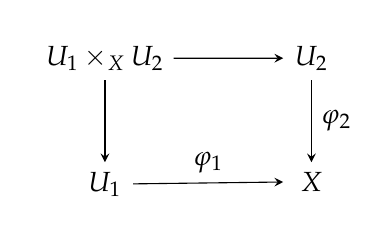
\begin{tikzpicture}
		\matrix (m) [matrix of math nodes,row sep=3em,column sep=4em,minimum width=2em]
		{
			U_1\times_X U_2 & U_2\\ 
			U_1 & X\\};
		\path[-stealth]
		(m-1-1) edge node [above] {} (m-1-2)
		(m-2-1) edge node [above]  {$\varphi_1$} (m-2-2)
		(m-1-1) edge node [right]  {} (m-2-1)
		(m-1-2) edge node [right] {$\varphi_2$} (m-2-2);
	\end{tikzpicture}
	\\
	having the obvious universal property. 
	
\end{definition}
\begin{definition}\label{site_defn}\cite{milne:lec}
	Let  $\mathscr C$  be a category. Suppose that  for each object $U$ of $\mathscr C$ there are  distinguished sets of families of morphisms $\left\{U_\iota \to U\right\}_{\iota\in I}$, called the \textit{coverings} of $U$, 
	satisfying the following axioms: 
	\begin{enumerate}
		\item[(a)] for any covering $\left\{U_\iota \to U\right\}_{\iota\in I}$ and any morphism $U \to V$ in $\mathscr C$, the fibre products 
		$U_\iota\times_U V$ exist, and $\left\{U_\iota\times_U V \to V\right\}_{\iota\in I}$ is a covering of $V$; 
		\item[(b)] if $\left\{U_\iota \to U \right\}_{\iota\in I}$ is a covering of $U$, and if for each $\iota \in I$, $\left\{V_{\iota j} \to U_\iota  \right\}_{j \in I_\iota}$	is a 
		covering of $U_\iota$, then the family $\left\{V_{\iota j }\to U\right\}_{\iota j}$ is a covering of $U$; 
		\item[(c)] for any $U$ in $\mathscr C$, the family $\left\{U\xrightarrow{\Id}U \right\}$ consisting of a single map is a covering of $U$. 
	\end{enumerate}
	The system of coverings is then called a \textit{Grothendieck topology}, and $\mathscr C$  together with 
	the topology is called a \textit{site}. If $\mathbf T$  
	is a site, then $\mathrm{Cat}\left( \mathbf T\right)\bydef \mathscr C$  denotes the underlying category. 
	
\end{definition}
\begin{example}\label{top_gro_exm}
	If $\sX$ is a topological space then one has a category of open subsets and their inclusions. If both $\sU_1, \sU_2 \subset \sX$ are open subsets then one can define a fibre product (cf. Definition \ref{pullback_defn}) by the following way
	$$
\sU_1\times_\sX \sU_2 \bydef \sU_1 \cap \sU_2.	
	$$
	If $\sU \subset \sX$ is an open subset then we assume that a family  $\left\{\sU_\iota \subset \sU\right\}_{\iota\in I}$, is a covering of $\sU$ (cf. Definition \ref{site_defn}) if and only if  $\sU = \cup_{\iota\in I}\sU_\iota$. This system of coverings is a specialization of Grothendieck topology. 
\end{example}
\begin{definition}\label{top_gro_definition}
In the situation of the Example \ref{top_gro_exm} one has a site $\mathbf T_{\sX}$ \textit{arising} from $\sX$.
\end{definition}

\begin{definition}\label{etale_presheaf_defn}\cite{milne:lec}
	A \textit{presheaf of sets} on a site $\mathbf T$ 
	is a contravariant functor $\mathscr F$ from $\mathrm{Cat}\left( \mathbf T\right)$ to the category of sets. Thus,  $\mathscr F$
	to each object $U$ in $\mathrm{Cat}\left( \mathbf T\right)$ 
	attaches a set $\mathscr F\left(U \right)$ , and to each morphism $\varphi: U \to V$
	in $\mathrm{Cat}\left( \mathbf T\right)$, a map $\mathscr F\left(\varphi\right):\mathscr F\left(V \right)\to \mathscr F\left(U \right)$. Note that the notion of a presheaf on $\mathbf T$ 
	does not depend on the 
	coverings. We sometimes denote $\mathscr F\left(\varphi\right)$ by $a \mapsto a|_U$.
	
\end{definition}
Similarly, a presheaf of (Abelian) groups or rings on $\mathbf T$ is a contravariant functor from
$\mathrm{Cat}\left( \mathbf T\right)$ to the category of (Abelian) groups or rings.
\begin{definition}\label{etale_sheaf_defn}\cite{milne:lec}
	A \textit{sheaf} on $\mathbf T$ 
	is a presheaf $\mathscr F$ 
	that satisfies the sheaf condition, that is a sequence 
	\be\label{etale_sheaf_eqn}
	\mathscr F \left(U\right) \to \prod_{\iota \in I} \mathscr F \left(U_\iota \right)\rightrightarrows  \prod_{\iota, j \in I\times I} \mathscr F \left(U_\iota \times_U U_j\right)
	\ee
	is exact for every covering $\left\{U_\iota \to U\right\}$. Thus $\mathscr F$ 
	is a sheaf if the map 
	$$
f \mapsto \left\{f|_{U_\iota }\right\}:\mathscr F \left(U\right) \to \prod_{\iota \in I} \mathscr F \left(U_\iota \right)
$$
	identifies $\mathscr F\left( U\right)$ with the subset of the product consisting of families $\left\{f|_{U_\iota }\right\}$ such that 
	$$
	f_\iota|_{U_\iota \times_U U_j}= f_j|_{U_\iota \times_U U_j}
	$$
	for all $\iota, j \in I$. 
	When $\mathbf T$ 
	is the site arising from a topological space then these definitions coincide with the 
topological ones. 
	
\end{definition}
\begin{definition}\label{forget_sheaf_defn}
There are categories $\mathbf{PreSh}\left(\mathbf T \right)$, $ \mathbf{Sh}\left(\mathbf T\right)$ of presheaves an sheaves. Moreover there is a \textit{forgetful functor} $\mathfrak{Forget} : \mathbf{Sh}\left(\mathbf T \right)\to \mathbf{PreSh}\left(\mathbf T \right)$.
\end{definition}

\begin{statement}\label{associated_sheaf_stmnt}\cite{johnstone:topos}
	There is an adjoint $\mathfrak{Ass} : \mathbf{PreSh}\left(\mathbf T  \right)\to \mathbf{Sh}\left(\mathbf T \right)$ to the  forgetful functor $\mathfrak{Forget} : \mathbf{Sh}\left(\mathbf T  \right)\to \mathbf{PreSh}\left(\mathbf T \right)$ (cf. Definition \ref{forget_sheaf_defn}).
\end{statement}	
\begin{defn}\label{associated_sheaf_defn}\cite{johnstone:topos}
	The given by the Statement  \ref{associated_sheaf_stmnt} functor $\mathfrak{Ass} : \mathbf{PreSh}\left(\mathbf T  \right)\to \mathbf{Sh}\left(\mathbf T \right)$  is said to be an  \textit{associated sheaf functor}.
\end{defn}
\begin{statement}\label{site_enough_stmt}\cite{johnstone:topos}
	%8.13$
	If $\mathbf T$ is a site then a category $\mathbf {Ab}\left(\mathbf T \right)$ of sheaves of Abelian groups has enough injectives.
\end{statement}
\begin{empt}
	The notion of \textit{topos} is explained in \cite{johnstone:topos}. Any topos is a category. If $\mathbf T$ is a site then a category  $\mathbf{Sh}\left(\mathbf T  \right)$ of sheaves of sets is a topos.
\end{empt}


\begin{definition}\label{grothendiek_topos_defn}\cite{johnstone:topos}
	A topos $\mathscr E$ is said to be a \textit{Grothendieck topos} if there exist a site $\mathbf T$ such that $\mathscr E$ is equivalent to a category  $\mathbf{Sh}\left(\mathbf T  \right)$ of sheaves of sets on $\mathbf T$.
\end{definition}

\begin{definition}\label{geom_mor_defn}\cite{johnstone:topos}
	% 1.16 
	If both $\mathscr E$, $\mathscr F$ are toposes then \textit{geometric morphism} $\mathscr F\xrightarrow{f}\mathscr E$ consists of a pair of functors $\mathscr F\xrightarrow{f_*}\mathscr E$  and $\mathscr E\xrightarrow{f^*}\mathscr F$ (called the \textit{direct} and \textit{inverse images}) such that $f^*$ is left adjoint to $f_*$ and $f^*$ is left exact. 
\end{definition}
%\begin{rem}\label{geom_mor_g_rem}\cite{johnstone:topos}
% 1.16 Grothendieck
%If both $\mathscr E$, $\mathscr F$ are Grothendieck toposes and  $\mathscr F\xrightarrow{f}\mathscr E$ is {geometric morphism} then direct image $f^*$ is left exact. 
%\end{rem}
\begin{definition}\label{constant_presheaf_defn}\cite{johnstone:topos}
If $X$ is an object of $\mathrm{Cat}\left( \mathbf T\right)$ (cf. Definition \ref{site_defn} then for any set $F$ there is a \textit{constant presheaf} $\mathscr P$ such that $\mathscr P\left( U\right) \bydef F$ and $\mathscr P\left( f\right) \bydef \Id_F$ for all $\mathrm{Cat}\left( \mathbf T\right)/X$-morphism $f: U\to V$.
We use a following notation
	\be\label{constant_presheaf_eqn}
	F_X \bydef \mathscr P.
	\ee
\end{definition}
\begin{thm}\label{zorn_thm}\cite{spanier:at} (Zorn's lemma). A partially ordered set in which every  simply ordered set has an upper bound contains maximal elements.
\end{thm}


\subsection{Cohomology of sheaves}\label{grothendieck_cohomology_section}
\paragraph{}
Here I follow to \cite{milne:lec}. Let $\mathbf T$ be a site, and let $X$ be an object of $\mathrm{Cat}\left( \mathbf T\right)$. The functor
\bean
\Ga\left(X, \cdot \right) : \mathbf {Ab} \left(\mathbf T \right) \to \mathbf {Ab} ,\\
\mathscr F \mapsto \mathscr F\left(X \right) 
\eean
of global sections is left exact, and we define $H^r\left(X,~ \cdot ~\right)$ to be its $r^{\text{th}}$ right derived functor. Explicitly, for a sheaf $\mathscr F$, choose an injective resolution (cf. Statement \ref{site_enough_stmt})
$$
0 \to \mathscr F \to \mathscr I^0\to \mathscr I^1\to \mathscr I^2 \to ...
$$
and apply the functor $\Ga\left(X, \cdot \right)$ to obtain a complex
\be\label{complex_eqn}
0 \hookto\Ga\left(X,\ \mathscr I^0  \right) \xrightarrow{\dl_0} \Ga\left(X, \mathscr I^1  \right) \xrightarrow{\dl_1} \Ga\left(X, \mathscr I^2  \right) \to ... 
\ee
which is no longer exact (in general). For any $r\ge 0$ the complex \eqref{complex_eqn} yields the $r^{\text{th}}$ \textit{cohomology
group}  
\be\label{etale_coh_eqn}
H^r\left(X,\ \mathscr F \right)\bydef\begin{cases}
	\ker \dl^0 & r = 0\\
 \ker~ \dl_{r} / \im~ \dl_{r - 1}  & r > 0
\end{cases},
\ee
which does not depend on choice of injective resolution up to isomorphism.

\begin{proposition}\label{spectral_sequence_prop}\cite{johnstone:topos}
	%8.17 
	Let $\mathscr F \xrightarrow{f} \mathscr E$ be a geometric morphism (cf. Definition \ref{geom_mor_defn}) between Grothendieck toposes (cf. Definition \ref{grothendiek_topos_defn}). Then
%	\begin{enumerate}		\item [(i)] 
	if $A$ is an Abelian group in $\mathscr E$ then we have a homomorphism $H^q\left(\mathscr E, A \right) \xrightarrow{} H^q \left(\mathscr F, f^*A\right)$ for each $q$ which is functorial in $f$ and natural in $A$.
	%	\item [(ii)] If $B$ is an Abelian group in $\mathscr F$ then we have a spectral sequence (Leray spectral sequence) $H^p\left(\mathscr E, R^qf_*\left(B \right) \right)\Rightarrow H^{p + q}\left(\mathscr F, B \right)$ which is natural in $B$.
%	\end{enumerate}
\end{proposition}
\begin{notation}\label{const_shef_coh_not}
	If  $F$ is an Abelian group and $F_X$ is a {constant presheaf} (cf. Definition \ref{constant_presheaf_defn}) then we use the following notation
	\be\label{const_shef_coh_eqn}
	\forall r\ge 0\quad H^r\left(X, F \right) \bydef H^r\left(X, \mathfrak{Ass} \left( F_X\right)  \right).
	\ee
	where $\mathfrak{Ass}$ means the associated sheaf functor (cf. Definition \ref{associated_sheaf_defn}).
\end{notation}




\subsection{\v{C}ech cohomology}\label{presheaf_cohomology_sec}
\paragraph{} Here I follow to \cite{milne:lec}. Let $\mathbf T$ be a site, and let $X$ be an object of $\mathrm{Cat}\left( \mathbf T\right)$. Let $\mathscr U \bydef \left\{U_\iota \to X\right\}_{\iota \in I}$ be  covering of $X$, and let $\mathscr P$ be a presheaf of Abelian groups. Define
\be\label{cech_eqn}
C^r\left( \mathscr U, \mathscr P\right)\bydef \prod_{\left(\iota_0,.... \iota_r\right) \in I^{r+1}} \mathscr P\left(U_{\iota_0,.... \iota_r} \right)\quad \text{where} \quad U_{\iota_0,.... \iota_r} \bydef U_{\iota_0}\times_X...\times_XU_{\iota_r}. 
\ee
For $s \in C^r\left( \mathscr U, \mathscr P\right)$ define $d^rs \in C^{r+1}\left( \mathscr U, \mathscr P\right)$ by the rule
$$
d^rs_{\iota_0,..., \iota_{r + 1}}\bydef \sum_{j = 0}^{r + 1}\left(-1 \right) \mathrm{res}_j\left(s_{\iota_0,..., \iota_{j-1},...,\iota_{j+1},..., \iota_{r + 1}} \right)  
$$
$\mathrm{res}_j$ is the restriction map corresponding to the projection map
$$
U_{\iota_0,..., \iota_{r + 1}}\mapsto U_{\iota_0,..., \iota_{j-1},...,\iota_{j+1},.., \iota_{r + 1}}.
$$
As in the classical case, one verifies by a straightforward calculation that
$$
C^\bullet\left( \mathscr U, \mathscr P\right) \bydef C^0\left( \mathscr U, \mathscr P\right) \to C^r\left( \mathscr U, \mathscr P\right) \xrightarrow{d_r} C^r\left( \mathscr U, \mathscr P\right)\to ...
$$
is a complex. Define
\be\label{cech_coh_eqn}
\check{H}^r\left( \mathscr U, \mathscr P\right) \bydef H^r\left(C^\bullet\left( \mathscr U, \mathscr P\right)   \right)= \begin{cases}
\ker d_0 & r = 0\\
\ker d_r / \im d_{r-1} & r > 0
\end{cases}. 
\ee
It is called the $r^{\text{th}}$ \textit{\v{C}ech cohomology group} of $\mathscr P$ relative to the covering $\mathscr U$.
Note that
$$
\check{H}^0\left( \mathscr U, \mathscr P\right)= \ker\left(\prod \mathscr P_\iota \rightrightarrows \prod \mathscr P_{\iota,j} \right) 
$$
Therefore, for a sheaf $\mathscr F$ one has
$$
\check{H}^0\left( \mathscr U, \mathscr F\right)=\Ga\left( \mathscr U, \mathscr F\right).
$$
A second covering $\mathscr V \bydef \left\{V_j\to X \right\}_{j \in J}$ of $X$ is called a \textit{refinement} of $\mathscr U$ if there is a
map $\tau : J\to I$ such that $V_j \to X$ factors through $U_{\tau_j}\to X$ for all $j \in J$ . The choice of
a $\tau$ and $X$-morphisms $\varphi_{j}: V_j \to U_{\tau_j}$ for each $j$ determines a map of complexes
\bean
\tau^\bullet: C^\bullet\left( \mathscr U, \mathscr P\right)\to C^\bullet\left( \mathscr V, \mathscr P\right),\\
\left( \tau^r s_{j_0,..., j_{r}} \right) \bydef s_{\tau j_0,..., \tau j_{r}}.
\eean
As in the classical case, one verifies that the map on cohomology groups
$$
\rho \left(\mathscr U, \mathscr V \right): \check{H}^r\left( \mathscr U, \mathscr P\right)\to \check{H}^r \left( \mathscr V, \mathscr P\right)
$$
is independent of all choices. We may pass to the limit over all coverings, and so obtain limits
\be\label{chech_eqn}
\check{H}^r\left(X, \mathscr P\right)\bydef \varinjlim_{\mathscr U}\check{H}^r\left( \mathscr U, \mathscr P\right).
\ee

\begin{defn}\label{chech_defn}\cite{bryl:loop,milne:lec}
	The  \textit{\v{C}ech cohomology groups} are given by equation \eqref{chech_eqn}.
\end{defn}
These groups  have the following properties:
\begin{enumerate}
	\item [(a)] $\check{H}^0\left(X, \mathscr F\right)= \Ga\left( X, \mathscr F\right)$ for any sheaf $\mathscr F$ on $X$;
	\item[(b)] $\check{H}^r\left(X, \mathscr I\right)$, $r > 0$, for all injective sheaves $\mathscr I$
\end{enumerate}
(cf \cite{milne:lec} for details).
\begin{empt}
	For any Abelian group $F$ one can define a constant presheaf $F_X$ of Abelian groups (cf. Definition \ref{constant_presheaf_defn}). 
	We use a following notation
	\be\label{etale_hom_a_eqn}
	\check{H}^r\left(X, F\right)\bydef \check{H}^r\left(X, F_X\right).
	\ee
\end{empt}
\section{Topological presheaves and sheaves}
\subsection{General theory}
\paragraph{}
The explained below definitions are specializations of   \ref{etale_presheaf_defn} and  \ref{etale_sheaf_defn} ones (cf. Example \ref{top_gro_exm}).
\begin{definition}\label{presheaf_defn}\cite{hartshorne:ag}
	Let $\sX$ be a topological space. A \textit{presheaf} $\mathscr F$ of Abelian groups on  $\sX$ consists of the data:
	\begin{itemize}
		\item[(a)] for every open subset $\sU \subseteq \sX$, an Abelian group $\mathscr F\left(\sU\right)$, and 
		\item[(b)] for every inclusion $\sV \subseteq \sU$ of open subsets of $\sX$, a morphism of Abelian groups $\rho_{\sU \sV}:\mathscr F\left(\sU\right) \to \mathscr F\left(\sV\right)$,\\
		subject to conditions
		\begin{itemize}
			\item [(0)] $\mathscr F\left(\emptyset \right)= 0$, where $\emptyset$ is the empty set,
			\item[(1)] $\rho_{\sU \sU}$ is the identity map, and
			\item[(2)] if $\mathcal W \subseteq \sV \subseteq \sU$ are three open sets, then $\rho_{\sU \mathcal W} = \rho_{\sV \mathcal W }\circ \rho_{\sU \sV}$.
		\end{itemize}
	\end{itemize}
\end{definition}

\begin{definition}\label{sheaf_defn}\cite{hartshorne:ag}
	A \textit{presheaf} $\mathscr F$ on  
	a topological space $\sX$ is a \textit{sheaf}  if it satisfies the following supplementary conditions:
	\begin{itemize}
		\item[(3)] If $\sU$ is an open set, and if $\left\{\sV_{\a}\right\}$ is an open covering of $\sU$, and if $s \in \mathscr F\left(\sU\right)$ is an element such that $\left.s\right|_{\sV_{\a}}= 0$ for all $\a$, then $s = 0$;
		\item[(4)] If $\sU$ is an open set, if $\left\{\sV_{\a}\right\}$ is an open covering of $\sU$ (i.e. $\sU = \cup\sV_\a$), and we have elements $s_\a$ for each $\a$, with property that for each $\al, \bt, \left.s_\a\right|_{\sV_{\a}\cap \sV_{\bt}}= \left.s_\bt\right|_{\sV_{\a}\cap \sV_{\bt}}$, then there is an element $s \in \mathscr F\left(\sU\right)$ such that $\left.s\right|_{\sV_\a} = s_\a$ for each $\a$.
	\end{itemize}
	(Note condition (3) implies that $s$ is unique).
\end{definition}



%\begin{definition}
%	A presheaf \ref{top_x_sheaf_defn} satisfying (4) of the Definition \ref{sheaf_defn} is called \textit{conjunctive} (for $\sU$). (cf. \cite{bredon:sheaf})
%\end{definition}
\begin{definition}\label{stalk_defn}\cite{hartshorne:ag}
	If $\mathscr F$ is a {presheaf} on $\sX$, and if $x$ is a point of $\sX$ we define the \textit{stalk} or the \textit{germ} $\mathscr F_x$ of $\mathscr F$ at $x$ to be the direct limit of groups $\mathscr F\left(\sU\right)$ for all open sets $\sU$ containing $x$, via restriction maps $\rho$.
\end{definition}

\begin{prdf}\label{sheaf_prdf}\cite{hartshorne:ag}
	Given a presheaf $\mathscr F$, there is a sheaf  $\mathscr F^+$ and a morphism $\th: \mathscr F \to \mathscr F^+$, with the property that for any sheaf  $\mathscr G$, and any morphism $\varphi: \mathscr F \to \mathscr G$, there is a unique morphism $\psi:\mathscr F^+\to \mathscr G$ such that $\varphi = \psi \circ \th$. Furthermore the pair $\left(\mathscr F^+, \th\right)$ is unique up to unique isomorphism. $\mathscr F^+$ is called the $\mathrm{sheaf~associated}$ to the presheaf $\mathscr F$. 
\end{prdf}
\begin{remark}
	The above Proposition is a specialization of the Statement \ref{site_enough_stmt}.
\end{remark}

\begin{exercise}\label{sheaf_etale_exer}\cite{hartshorne:ag}
	%1.13. 
	\textit{
		\'Espace Etal\'e of a Presheaf}. %(This exercise is included only to establish the connection between our definition of a sheaf and another definition often found in the literature. See for example Godement [1, Ch. II, �1.2].)
	Given a presheaf $\mathscr F$ on $\sX$, we define a topological space $\mathrm{Sp\acute{e}}\left(\mathscr F \right)$ , called the \textit{
		\'espace etal\'e} of a presheaf of $\mathscr F$ as 
	follows. As a set, $\mathrm{Sp\acute{e}}\left(\mathscr F \right)= \bigcup_{x\in\sX} \mathscr F_x$. We define a projection map $p: \mathrm{Sp\acute{e}}\left(\mathscr F \right)\to \sX$
	by sending $s_x\in \mathscr F_x$ to $x$. For each open set $\sU\subset\sX$ and each section $s\in \mathscr F\left(\sU \right)$  we 
	obtain a map: $\overline{s}: \sU \to  \mathrm{Sp\acute{e}}\left(\mathscr F \right)$ by sending $x \mapsto s_x$, its stalk at $x$. This map has the property that 
	$p\circ \overline{s}= \Id_\sX$, in other words, it is a "section" of $p$ over $\sU$. We now 
	make $\mathrm{Sp\acute{e}}\left(\mathscr F \right)$ into a topological space by giving it the strongest topology such that 
	all the maps $\overline{s}: \sU \to  \mathrm{Sp\acute{e}}\left(\mathscr F \right)$ for all $\sU$ and all $s\in \mathscr F\left(\sU \right)$ , are continuous. Now 	show that the sheaf $\mathscr F^+$ associated to $\mathscr F$ can be described as follows: for any 
	open set $\sU\subset \mathscr F$, $\mathscr F\left(\sU \right)$ is the set of continuous sections of $\mathrm{Sp\acute{e}}\left(\mathscr F \right)$ over $\sU$. In 
	particular, the original presheaf $\mathscr F$ was a sheaf if and only if for each $\sU\subset \sX$,  $\mathscr F\left(\sU \right)$ is 
	equal to the set of all continuous sections of $\mathrm{Sp\acute{e}}\left(\mathscr F \right)$ over $\sU$. 
\end{exercise}	
\begin{exercise}\label{sheaf_etale_open_exer}

Let $s \in \mathscr F\left(\sU\right)$ be a section. Prove following statements.
\begin{enumerate}
	\item The set 
	\be\label{sheaf_u_s_eqn}
\mathscr U_s\bydef \left\{s_x\right\}_{x \in \sU}
	\ee
is open subset  of the \'espace etal\'e  of $\mathrm{Sp\acute{e}}\left(\mathscr F \right)$ of the presheaf $\mathscr F$.
	\item The family  of all given by the equation \eqref{sheaf_u_s_eqn} sets $\mathscr U_s$ is basis of the topology of  $\mathrm{Sp\acute{e}}\left(\mathscr F \right)$.
	\item The natural continuous map $\mathrm{Sp\acute{e}}\left(\mathscr F \right)\to\sX$ is local homeomorphism.
	\end{enumerate}
\end{exercise}

\begin{definition}\label{sheaf_inv_im_defn}\cite{hartshorne:ag}
	Let $f: \sX\to \sY$ be a continuous map of topological spaces. For any sheaf  $\mathscr F$ on $\sX$, we define the \textit{direct image} sheaf  $f_*\mathscr F$ on $\sY$ by $\left(f_*\mathscr F\right)\left(\sV\right)= \mathscr F\left(f^{-1}\left(\sV\right)\right)$ for any open set $\sV \subseteq \sY$. For any sheaf  $\mathscr G$ on $\sY$, we define the \textit{inverse image} sheaf  $f^{*}\mathscr G$ on $\sX$ be the sheaf  associated to the presheaf  $\sU \mapsto \lim_{\sV \supseteq f\left(\sU\right)} \mathscr G\left(\sV\right)$, where $\sU$ is any open set in $\sX$, and the limit is taken over all open sets $\sV$ of $\sV$ containing $f\left(\sU\right)$.
\end{definition}

\begin{remark}\label{geometric_morphism_rem}\cite{johnstone:topos}
	%1.17
	If $f : \sX \to \sY$ is a continuous map then a given by the Definition \ref{sheaf_inv_im_defn} pair  of functors $f_*$ and $f^{*}$ rise a geometric morphism (cf. Definition \ref{geom_mor_defn}) $\mathbf{Sh}\left(\sX\right)\to \mathbf{Sh}\left(\sY\right)$ between categories of sheaves. 
\end{remark}
\begin{exercise}\label{dir_image_exer}
	Let $f : \sX \to \sY$ be a continuous map, and let $F$ be a set. Prove that if  	both $F_\sX$ and $F_\sY$ are constant presheaves  (cf. Definition \ref{constant_presheaf_defn}) on $\sX$ and $\sY$ 
	then one has:
	\begin{enumerate}
		\item there is a natural isomorphism of sheaves
		\bean\label{dir_image_eqn}
		\mathfrak{Ass}\left( F_\sY\right) \cong f_*\mathfrak{Ass}\left( F_\sX\right)
		\eean
		where 
		$\mathfrak{Ass}$  means the associated sheaf functor (cf. Definition \ref{associated_sheaf_defn}) and 	
		$f_*$ means the direct image (cf. Definition \ref{sheaf_inv_im_defn}),
		\item if $f$ ia a local homeomorphism then there is a natural isomorphism of sheaves
		\be\label{inv_image_eqn}
		\mathfrak{Ass}\left( F_\sX\right) \cong f^*\mathfrak{Ass}\left( F_\sY\right)
		\ee
	where	$f^*$ means the  inverse image (cf. Definition \ref{sheaf_inv_im_defn}).
	\end{enumerate}
\end{exercise}
\begin{definition}\label{sheaf_morphism_defn}\cite{hartshorne:ag}
	If $\mathscr F$  and $\mathscr G$ are presheaves on $\sX$, a \textit{morphism} $\varphi:\mathscr F\to\mathscr G$  consists 
	of a morphism of Abelian groups $\varphi_\sU:\mathscr F\left( \sU\right) \to\mathscr F\left( \sU\right)$ for each open set 
	$\sU$, such that whenever $\sV\subset\sU$ is an inclusion, the diagram 
	\newline
	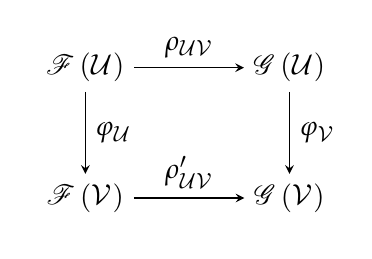
\begin{tikzpicture}
		\matrix (m) [matrix of math nodes,row sep=3em,column sep=4em,minimum width=2em]
		{
			\mathscr F\left( \sU\right)   & \mathscr G\left( \sU\right)\\
			\mathscr F\left( \sV\right)    & \mathscr G\left( \sV\right)\\
		};
		\path[-stealth]
		(m-1-1) edge node [above] {$\rho_{\sU\sV}$} (m-1-2)
		(m-1-1) edge node [right] {$\varphi_\sU$} (m-2-1)
		(m-1-2) edge node [right] {$\varphi_\sV$} (m-2-2)
		(m-2-1) edge node [above] {$\rho'_{\sU\sV}$} (m-2-2);
	\end{tikzpicture}
	\\
	is commutative, where $\rho_{\sU\sV}$ and $\rho'_{\sU\sV}$ are the restriction maps in $\mathscr F$  and $\mathscr G$. If $\mathscr F$  and $\mathscr G$ are sheaves on $\sX$, we use the same definition for a morphism 
	of sheaves. An isomorphism is a morphism  which has a two-sided inverse. 
\end{definition}
\begin{empt}\label{open_sheaf_empt}
For any topological space $\sX$ there is a \textit{sheaf of stalks of open sets} $\Om_\sX$ on $\sX$ (cf. \cite{goldblatt:topoi})
such that
\bean
\Om_\sX \left(\sU \right)  \bydef  \text{the family of all open subsets of }\sU;\\
\rho_{\sU \sV}: \Om_\sX\left(\sU \right) \to \Om_\sX\left(\sV \right), \quad \mathcal W \mapsto \mathcal W \cap \sV.
\eean
\end{empt}

\subsection{Cohomology}
\paragraph{}
The described below theories are specializations of described in sections \ref{grothendieck_cohomology_section} and \ref{presheaf_cohomology_sec} ones (cf. Example \ref{top_gro_exm}).
%\begin{lemma}\cite{hartshorne:ag}
%	Let $\sX$ be a topological space, and $\mathscr U$ an open covering of $\sX$. Then for any sheaf $\mathscr U$ on $\sX$ and	for each $r \ge 0$ there is a natural map, functorial in $\mathscr F$.
%	$$
%	\check{H}^r\left(\mathscr U, \mathscr F \right) \to H^r\left( \sX, \mathscr F\right) 
%	$$
%	where both $\check{H}^r$ and $H^r$ are given by the equations \eqref{cech_coh_eqn} and \eqref{etale_coh_eqn} respectively.
%\end{lemma}
%\begin{remark}
%From the above lemma and the equation  \ref{chech_eqn} for each $r\ge 0$ one has a homomorphism
%$$
%\check{H}^r\left(\sX, \mathscr F \right) \to H^r\left( \sX, \mathscr F\right).
%$$
%\end{remark}
\begin{empt}
	If $f: \sX\to\sY$ is a continuous map  $\mathscr U = \left\{\sU_\iota\right\}_{\iota} \in I$ is a covering of $\sY$ (cf. Definition \ref{site_defn} and Example \ref{top_gro_exm}) then a family $f^{-1}\left(\mathscr U \right) \bydef \left\{f^{-1}\left( \sU_\iota\right) \right\}_{\iota} \in I$ is a covering of $\sX$. Let $F$ be a Abelian group, and let $F_\sX$, $F_\sY$ be a corresponding constant presheaves (cf. Definition \ref{constant_presheaf_defn}) on $\sX$ and $\sY$.  Following equation
	\be\label{top_cech_eqn}
	C^r\left( \mathscr U,  F_\sY\right)\bydef \prod_{\left(\iota_0,.... \iota_r\right) \in I^{r+1}}  F_\sY\left(\sU_{\iota_0,.... \iota_r} \right)\quad \text{where} \quad \sU_{\iota_0,.... \iota_r} \bydef \sU_{\iota_0}\cap...\cap \sU_{\iota_r}. 
	\ee
	is a specialization of \eqref{cech_eqn} one (cf. Example \ref{top_gro_exm}). For any $\left(\iota_0,.... \iota_r\right) \in I^{r+1}$ one has an isomorphism
	$$
	F_\sY\left(\sU_{\iota_0,.... \iota_r} \right)\cong F_\sX\left(f^{-1}\left( \sU_{\iota_0,.... \iota_r} \right)\right) \cong F.
	$$
	Above isomorphisms yield an isomorphism
	$$
	C^r\left( \mathscr U, F_\sY\right)\xrightarrow{\approx} C^r\left( f^{-1}\left( \mathscr U\right) , F_\sX\right)
	$$
    So there is an isomorphism
    $$
 \varinjlim_{\mathscr U}\check{H}^r\left( \mathscr U, F_\sY\right)\xrightarrow{\approx}\varinjlim_{\mathscr U}\check{H}^r\left(f^{-1}\left(  \mathscr U\right) , F_\sX\right).
    $$
On the other hand from   \eqref{chech_eqn}  it follows that there are homomorphisms
\bean
\check{H}^r\left(f^{-1}\left(  \mathscr U\right) , F_\sX\right)\to \check{H}^r\left(\sX , F_\sX\right),\\
\varinjlim_{\mathscr U} \check{H}^r\left(f^{-1}\left(  \mathscr U\right), F_\sX\right)\to \check{H}^r\left(\sX , F_\sX\right)
\eean
so one has a homomorphism
$$
\varinjlim_{\mathscr U} \check{H}^r\left(  \mathscr U, F_\sY\right)\to \check{H}^r\left(\sX , F_\sX\right)
$$
and applying \eqref{chech_eqn} one can obtain a natural homomorphism
	$$
	\check{H}^r\left(f\right):\check{H}^r\left(\sY, F_\sY \right)\to \check{H}^r\left(\sX, F_\sX \right)\quad r \ge 0.
	$$
	The details of the construction of the homomorphism $\check{H}^r\left(f\right)$  are explained in \cite{eust}. Using the Notation \ref{constant_presheaf_defn} one has homomorphisms
	\be\label{cech_hom_eqn}
	\begin{split}
		\check{H}^r\left(f\right):\check{H}^r\left(\sY, F \right)\to \check{H}^r\left(\sX, F \right)\quad r \ge 0,\\
		\check{H}^\bullet\left(f\right):\check{H}^\bullet\left(\sY, F \right)\to \check{H}^\bullet\left(\sX, F \right).
	\end{split}
	\ee
	If both $\sX \xrightarrow{f}\sY$ and $\sY \xrightarrow{g}\sZ$ are continuous maps then from this construction it turns out that
	\be\label{cech_hom_comp_eqn}
	\begin{split}
		\check{H}^\bullet\left(g\circ f\right)= \check{H}^\bullet\left( f\right)\circ \check{H}^\bullet\left(g\right):\check{H}^\bullet\left(\sZ, F \right)\to \check{H}^\bullet\left(\sX, F \right)
	\end{split}
	\ee
	
\end{empt}

\begin{empt}\label{tens_prop_c_empt}\cite{bryl:loop}
\v{C}ech cohomology has the advantage of allowing an easy and explicit construction of a \textit{cup}-\textit{product}
$$
\check{H}^p\left(\mathscr U,  \mathscr F\right) \otimes \check{H}^q\left(\mathscr U,  \mathscr G\right)\to \check{H}^p\left(\mathscr U,  \mathscr F\otimes \mathscr G\right).
$$
		Here $\mathscr F$ and $\mathscr G$ are sheaves of Abelian groups on $\sX$, and the \textit{tensor product}-\textit{sheaf}
	 $\mathscr F\otimes \mathscr G$ is the sheaf associated to the presheaf $\sU \mapsto \mathscr F(\sU)\otimes \mathscr G(\sU)$. The 
		stalk (cf. Definition \ref{stalk_defn}) at $x$ of $\mathscr F\otimes \mathscr G$ is $\mathscr F_x\otimes \mathscr G_x$. The cup-product will be defined from a 
		morphism of complexes. We first need the notion of tensor product $A^\bullet \otimes  B^\bullet$
		of two complexes; this is the total complex of the double complex $A^\bullet \otimes  B^\bullet$. 
		So the degree $n$-term of $A^\bullet \otimes  B^\bullet$ is $\oplus A^p\otimes B^{n-p}$. The differential in $A^\bullet \otimes  B^\bullet$  
		is 
		$$
	d \left(a \otimes b\right)	\bydef \left(da\right)\otimes b + \left(-1\right)^p a \otimes db
		$$
		
	for $a\in A^p$, $b \in B^q$. We have the obvious 
		map 
	$$
\otimes :H^p\left(A^\bullet\right)\otimes H^q\left(B^\bullet\right)\to H^q\left(A^\bullet\ox B^\bullet\right).	
	$$	
	We now return to the sheaves $\mathscr F$ and $\mathscr G$ of Abelian groups on $\sX$. We 
		have the complexes $C^\bullet\left(\mathscr U,  \mathscr F\right)$ and $C^\bullet\left(\mathscr U,  \mathscr G\right)$.  The interesting part is the 
		construction of a morphism of complexes 
	$$
\phi: C^\bullet\left(\mathscr U,  \mathscr F\right)\otimes C^\bullet\left(\mathscr U,  \mathscr G\right)\mapsto C^\bullet\left(\mathscr U,  \mathscr F\otimes  \mathscr G\right).
	$$
		For $\a \in C^\bullet\left(\mathscr U,  \mathscr F\right)$ and $\bt \in C^\bullet\left(\mathscr U,  \mathscr G\right)$, we put 
	$$
	\phi:\left( \a \otimes \bt \right)_{\iota_0,..., \iota_{p + q}} \bydef \a_{\iota_0,...,\iota_p}\otimes  \bt_{\iota_{p},..., \iota_{p+q}}.
	$$
			One checks easily that $\phi$ is indeed a morphism of complexes. The induced map on cohomology gives the cup-product on \v{C}ech 
			cohomology. For $\a$ degree $p$ \v{C}ech cocycle with coefficients in $\mathscr F$ and $\bt$
			degree $q$ \v{C}ech cocycle with coefficients in $\mathscr G$, we have 
			$$
		\left(\a \smile\bt \right)_{\iota_0,..., \iota_{p + q}}\bydef  \a_{\iota_0,...,\iota_p}\otimes  \bt_{\iota_{p},..., \iota_{p+q}}.
		$$
			The cup-product has the following properties. 
		\end{empt}
		\begin{proposition}\label{cup_ass_prop}\cite{bryl:loop} Following conditions hold.
		%	1.3.7. Proposition. 
		\begin{enumerate}
			\item[(i)] The cup-product is associative, i.e., for $\a \in \check{H}^p\left(\mathscr U,  \mathscr F\right)$,  $\bt \in \check{H}^q\left(\mathscr U,  \mathscr G\right)$, $\ga \in \check{H}^r\left(\mathscr U,  \mathscr H\right)$
	 we have 
	 $$
\a \smile \left( \bt \smile \ga\right) 	= \left( \a \smile \bt\right) \smile \ga. 
	 $$
	 	\item[(ii)]	 The \textit{cup}-\textit{product} is \textit{graded}-\textit{commutative}. If $\a \in \check{H}^p\left(\mathscr U,  \mathscr F\right)$,  $\bt \in \check{H}^q\left(\mathscr U,  \mathscr G\right)$, we have 
$$
\a \smile \bt =\left( -1\right)^p  \bt \smile \a.
$$			
			
		\end{enumerate}
			
	\end{proposition}
	\begin{empt}
		Let $\sX$ be a topological space. If $F$ be an Abelian group then there is, a corresponding constant presheaf  $F_\sX$ (cf. Definition \ref{constant_presheaf_defn}) on $\sX$. A  presheaf $F_\sX\otimes F_\sX$ on $\sX$ is a constant presheaf of a group $F\otimes_Z F$.  An isomorphism $A \otimes_\Z A \cong  A$ naturally yields an isomorphism $F_\sX\otimes F_\sX\cong  F_\sX$ of sheaves which induces an isomorphism
		$$
\phi: \check{H}^\bullet\left(\sX, F_\sX\otimes F_\sX \right)\cong \check{H}^\bullet\left(\sX, F_\sX \right).
		$$
		Using the cup product and homomorphism $\phi$ one has a map
	$$
	\check{H}^\bullet\left(\sX, F_\sX \right)\otimes \check{H}^\bullet\left(\sX, F_\sX \right) \to \check{H}^\bullet\left(\sX, F_\sX \right).
	$$
	So we have proved the following.	
	\end{empt}
	
	\begin{lem}\label{gr_ring_lem}
		Let $\sX$ be a topological space. If $F$ is an Abelian group then any isomorphism $F \otimes_\Z F \cong  F$ yields a product
		\bean
		\smile: \check{H}^\bullet\left(\sX, F \right)\otimes \check{H}^\bullet\left(\sX,F \right) \to \check{H}^\bullet\left(\sX,F \right)
		\eean
		where the notation \eqref{etale_hom_a_eqn} is used. So $\check{H}^\bullet\left(\sX, F\right)$ becomes an associative and graded-commutative ring.
	\end{lem}
	
	\begin{exercise}\label{ring_homo_exer}
	Let  $F$ be an Abelian group with a homomorphism $F \otimes_\Z F \cong F$. Prove that a given by \eqref{cech_hom_eqn} map $\check{H}^\bullet\left(f\right):\check{H}^\bullet\left(\sY, F \right)\to \check{H}^\bullet\left(\sX, F \right)$ is a homomorphism of rings.
	\end{exercise}

\section{$C^*$-algebras}
\paragraph*{}  A notion of $C^*$-algebra is explained in \cite{murphy, pedersen:ca_aut, rae:ctr_morita}.

	\begin{thm}(Dauns Hofmann)\label{dauns_hofmann_thm}\cite{pedersen:ca_aut}
	For each $C^*$-algebra $A$ there is the natural isomorphism from the center of $M\left( A\right)$ onto the class of bounded continuous  functions on $\check{A}$. 
\end{thm}


\subsection{Hereditary $C^*$-subalgebras}

	\begin{definition}\label{hered_defn}\cite{pedersen:ca_aut}
	A cone $M$ in the positive part of $C^*$-algebra $A$ is said to be \textit{hereditary} if $0 \le x \le y$, $y \in M$ implies $x \in M$ for each $x \in A$. A $C^*$-subalgebra $B$ of $A$ is \textit{hereditary} if $B_+$ is hereditary in $A_+$.
\end{definition}
%\begin{lemma}\label{hered_lem}\cite{murphy}
%	Let $B$ be a $C^*$-subalgebra of $C^*$-algebra $A$. Then $B$ is hereditary in $A$ if and only if $bab' \in B$ for all $b, b' \in B$ and $a \in A$.
%\end{lemma}
\begin{lemma}\label{hered_ideal_lem}\cite{murphy}
	Let $A$ be a $C^*$-algebra.
	\begin{enumerate}
		\item[(i)] If $L$ is a closed left ideal in $A$ then $L\cap L^*$ is a hereditary $C^*$-subalgebra of $A$. The map $L \mapsto L\cap L^*$ is the bijection from the set of closed left ideals of $A$ onto the the set of hereditary $C^*$-subalgebras of $A$.
		\item[(ii)] If $L_1, L_2$ are closed left ideals, then $L_1 \subseteq L_2$ is and only if $L_1\cap L_1^* \subset L_2\cap L_2^*$.
		\item[(iii)] If $B$ is a hereditary $C^*$-subalgebra of $A$, then the set 
\be\label{left_ideal_eqn}
		L\left(B \right) = \left\{\left.a \in A~\right| a^*a \in B\right\}
\ee
		is the unique closed left ideal of $A$ corresponding to $B$.
	\end{enumerate}
\end{lemma}


\begin{remark}\label{hered_rem}\cite{murphy}
	Obviously, $0$ and
	$A$ are hereditary $C^*$-subalgebras of $A$, and any intersection of hereditary
	$C^*$-subalgebras is one also. 
	
\end{remark}
\begin{definition}\label{hered_generated_defn}\cite{murphy}
	The hereditary $C^*$-subalgebra \textit{generated} by a
	subset $S$ of $A$ is the smallest hereditary $C^*$-subalgebra of $A$ containing $S$.
\end{definition}


\begin{lemma}\label{hered_repr_lem}\cite{pedersen:ca_aut}
	%4.1.5. LEMMA. 
	Let $B$ be a hereditary $C^*$-subalgebra of $A$. For each irreducible 
	representation $\pi: A \to B\left( \H\right)$  such that $B \not\subset\ker\pi$ the map $\pi|_B: B \to \pi\left(B \right)\H$  is an irreducible 
	representation of $B$. 
	
\end{lemma}

\begin{theorem}\label{left_ideal_thm}\cite{murphy}
	%3.1.2. Theorem.
	If $L$ is a closed left ideal in a $C^*$-algebra $A$, then there
	is an increasing net $\left\{u_\la\right\}_{\la\in\La}$ of positive elements in the closed unit ball of
	$L$ such that $a = \lim_{\la\in \La}au_\la $ for all $a\in L$.
\end{theorem}


\subsection{Continuous trace $C^*$-algebras}

\begin{definition}\label{type_i0_defn}\cite{pedersen:ca_aut}
	% 6.1
A positive element $a$ in a $C^*$-algebra $A$ is \textit{Abelian} if 
the hereditary $C^*$-subalgebra generated by $a$, i.e. the norm closure of $aAa$, is 
commutative. If $A$ is  generated (as a $C^*$-algebra) 
by its Abelian elements we say that it is of \textit{type} $I_0$. 
\end{definition}
\begin{lemma}\label{type_i0_lem}
%6.1.3. LEMMA 
A positive element $a$ in a $C^*$-algebra $A$ is Abelian if and only if $\dim \pi\left(a \right)\le 1$ for every irreducible representation $\pi: A \to B\left(\H \right)$. 
\end{lemma}	
\begin{definition}\label{continuous_trace_c_alt_defn}\cite{rae:ctr_morita}
	%Definition 5.13. 
	A \textit{continuous-trace} $C^*$-\textit{algebra} is a $C^*$-algebra $A$ with Hausdorff
	spectrum $\sX$ such that, for each $x_0\in\sX$ there are a neighborhood $\sU$ of $x_0$ and $a\in A$ such that $\rho_{ x}\left( a\right) $ is a rank-one projection for all $x \in \sU$, where $\rho_{ x}: A \to B\left(\H_x\right)$ is a corresponding to $x$ irreducible representation.
\end{definition}
\begin{remark}\label{ctr_gen_rem}\cite{pedersen:ca_aut}
Any {continuous-trace} $C^*$-{algebra}  $A$ is of type $I_0$.
\end{remark}

\begin{lemma}\label{ctr_rep_eq_lem}\cite{rae:ctr_morita}
	Suppose $A$ is a $C^*$-algebra with Hausdorff spectrum $\mathcal{X}$ and for all $x \in \sX$ $\pi_x : A \to B\left(\H_x \right)$ is a corresponding  to $x$ irreducible representation then for each $a \in A$ the function $x \mapsto \left\|\pi_x\left(a \right) \right\|$ is continuous on  $\mathcal{X}$, vanishes at infinity and has sup-norm equal to $\left\| a\right\|$. 
\end{lemma}
\begin{rem}\label{ctr_spe_rem}
	From the Lemma \ref{hered_repr_lem} it follows that if $A$ 	 has continuous trace and $\sX$ is a spectrum of $A$ then a spectrum $\sX_B$ of any hereditary subalgebra $B$ is an open subset of $\sX$ (cf.  \cite{pedersen:ca_aut} for details).
\end{rem}


\begin{proposition}\label{ctr_lt_prop}\cite{cuntz_meyer_ros:bivariant}
	%Proposition 9.3. 
	Let $\H$ be a Hilbert space, and let $\K \bydef \K\left(\H \right)$  be the algebra of
	compact operators on $\H$. Then every irreducible *-representation of $\K$ is unitary
	equivalent to the standard representation of $\K$ on $\sH$, and every $*$-automorphism
	of $\K$ is given by conjugation by a unitary operator on $\H$. The *-automorphism
	group of $\K$ can be identified with the topological group $PU\bydef U/\T$ the
	projective unitary group of $\H$, with the quotient topology from the strong operator
	topology on $U\left(\H\right)$.
\end{proposition}

\begin{proposition}\label{ctr_bundle_prop}\cite{cuntz_meyer_ros:bivariant}
	%Proposition 5.59. 
%Theorem 9.9 
(Dixmier�Douady). 
Any stable separable algebra A of continuous
trace over a second-countable locally compact Hausdorff space $\sX$ is isomorphic to
$\Ga_0\left( \sX, \sF\right)$ , the sections vanishing at infinity of a locally trivial bundle of algebras
over $\sX$, with fibres $\K$ and structure group $\Aut(\K) = PU = U/\T$. Classes of
such bundles are in natural bijection with the \v{C}ech cohomology group $\check{H}^3\left(\sX, \Z \right)$.
The 3-cohomology class $\dl\left( A\right)$  attached to (the stabilization of) a continuous-trace
algebra A is called its Dixmier�Douady class.
\end{proposition}
\begin{proof}
Principal $PU$-bundles over $\sU$ are thus classified by
$\left[\sX, BPU\right] = \left[\sX, K\left( \Z, 3\right) \right] = H^3\left(\sX, \Z \right)$. 
The details of the proof are presented in \cite{cuntz_meyer_ros:bivariant}.
\end{proof}

\begin{proposition}\label{ctr_d_prop}\cite{cuntz_meyer_ros:bivariant}
%Proposition 9.11 (P. Green [51,96,104]). 
Let $\sX$ be a second-countable locally compact
Hausdorff space, and let $A$ and $B$ be stable algebras of continuous trace over $\sX$.
Then $A \times_\sX B$ is also a stable continuous-trace algebra over $\sX$, and the Dixmier�Douady class $\dl \left(A \otimes_\sX B \right)$  of $A \times_\sX B$ is given by $\dl(A) + \dl(B)$. The Dixmier�Douady class of the opposite algebra $A^{\mathrm{op}}$ is given by $\dl\left( A^{\mathrm{op}}\right)=$ - $\dl\left( A\right)$ , so that
$A\times_\sX  A^{\mathrm{op}}= C_0\left(\sX, \K\right)$.
\end{proposition}
\begin{notation}\label{ctr_not}
	If $\sX$ is a locally compact Hausdorff space then we denote by $CT\left(\sX, \dl \right)$ the stable
	continuous-trace algebra  with Dixmier�Douady class $\delta \in \check{H}^3\left(\sX,\Z \right)$. From the Proposition \ref{ctr_d_prop} it follows that
	\be\label{bundle_prod_iso}
\varphi_{\dl \rho}	:CT\left(\sX, \dl \right)\times_\sX CT\left(\sX, \rho \right)\cong CT\left(\sX, \dl +\rho\right).
	\ee
\end{notation}
\begin{proposition}\label{ctr_cup_prop}\cite{cuntz_meyer_ros:bivariant}
%Proposition 9.17.
There are natural homomorphisms
\bea\label{ka_eqn}
K_\bullet\left( CT\left(\sX, \dl \right)\right)\otimes_\Z K_\bullet\left( CT\left(\sX, \rho \right)\right) \to K_\bullet\left( CT\left(\sX, \dl + \rho\right)\right),\\
\label{kx_eqn}
K_\bullet\left( CT\left(\sX, 0 \right)\right)\cong K^\bullet\left( \sX\right),
\eea
where $K_\bullet\left( CT\left(\sX, \dl \right)\right)$ means $K$-theoretic groups of $C^*$-algebra $ CT\left(\sX, \dl \right)$ and $K^\bullet\left( \sX\right)$ means $K$-theoretic groups of the space $\sX$.
\end{proposition}

\section{Groupoids, foliations,  and $C^*$-algebras}\label{foliations_sec}
\subsection{Groupoids and their $C^*$-algebras}
\paragraph*{}
A groupoid is a small category with inverses, or more explicitly:
\begin{definition}\label{groupoid_defn}\cite{renault:gropoid_ca}
	% 104
	A \textit{groupoid} consists of a set $\G$, a distinguished subset $\G^0\subset\G$, two maps
	$r, s : \G\to \G^0$ and a law of composition
	$$
	\circ: \G^2\bydef\left\{\left.\left(\ga_1,\ga_2 \right) \in \G\times\G~\right| s\left(\ga_1\right)= r\left(\ga_2\right)\right\}\to \G
	$$
	such that
	\begin{enumerate}
		\item $s\left(\ga_1\circ\ga_2\right)=s\left(\ga_2\right), \quad r\left(\ga_1\circ\ga_2\right)=r\left(\ga_1\right)\quad \forall\left(\ga_1, \ga_2 \right) \in \G$
		\item $s\left(x\right)=r\left(x\right)=x \quad\forall x\in\G^0$
		\item $\ga\circ s\left(\ga\right)= r\left(\ga\right)\circ\ga = \ga\quad \forall\ga\in\G$
		\item $\left( \ga_1\circ\ga_2\right) \circ\ga_3=\ga_1\circ\left( \ga_2\circ\ga_3\right) $
		\item Each $\ga \in\G$ has a two-sided inverse $\ga^{-1}$, with $\ga\circ\ga^{-1}=r\left(\ga\right)$, $\ga^{-1}\circ\ga=r\left(\ga\right)$.
	\end{enumerate}
	The maps $r$, $s$ are called the \textit{range} and \textit{source} maps.
\end{definition}

\begin{definition}\label{groupoid_reduction_defn}\cite{renault:gropoid_ca}
	Let $\G$ be a groupoid, and let $E$ be a subset of $G^0$.
	A subgroupoid 
	$$
	\G^E_E \bydef \left\{x \in G | r(x), s(x)\in E\right\}
	$$
	with unit space $E$ is said to be  the \textit{reduction} 
	of $\G$ by $E$.
\end{definition}
\begin{empt}\label{cycle_empt}\cite{renault:gropoid_ca}
	The notion of \textit{topological groupoid} is explained in \cite{renault:gropoid_ca}. 
	If $F$ is an Abelian group then then for all $r \ge 0$ there is $r^{\text{th}}$ \textit{cohomology group} $H^r\left( \G, F\right)$. Any element of $H^2\left( \G, F\right)$ can be represented  by a 2-\text{cycle} $\a \in Z^2\left(\G, F \right)$. Note that a 2-cycle $\a$ is a map   $\G^2 \to F$. If $\G$ is a topological groupoid and  $F$ is a topological group then we assume that the map $\a$ is continuous. We write $\left[\a\right]\in H^r\left( \G, F\right)$.
\end{empt}
\begin{remark}\label{hoto_rem}
	If both $\a', \a''\in \Z^2\left(\G, F \right)$ are homotopic 2-cocycles  then  $\left[\a'\right]= \left[\a''\right]\in H^2\left( \G, F\right)$.
\end{remark}
\begin{empt}\label{groupoid_haar_empt}\cite{renault:gropoid_ca}
	The notion of  \textit{left Haar system} on locally compact groupoid is explained in \cite{renault:gropoid_ca}. Let $\G$ be a locally compact groupoid with left Haar system $\left\{\la^u\right\}$ and let $\a$ be a continuous 2-cocycle in $Z^2\left(\G, \T\right)$. For $f ,g \in C_c(\G )$, let us define
	\bea\label{groupoid_*_c_eqn}
	f * g \left(x\right)\bydef 
	\int f ( x y ) g \left( y^{-1}\right)\a\left(xy, y^{-1} \right) d\la^{d(x)}(y),\\
	\label{groupoid_inv_c_eqn}
	f^* ( x ) \bydef\overline{f ( x^{ -1})}, 	
	\eea
	so $ C_c(\G )$ becomes a *-algebra, we denote it by $C_c\left( \G, \a\right)$. Denote by $C^*_r\left( \G, \a\right)$ a completion of  $C_c\left(\G, \a\right)$ with respect to the following $C^*$-norm
	\be\label{groupoid_norm_eqn}
	\left\|a \right\| \bydef \sup_{\pi \in \text{Irr}\left(C_c\left(\G\right)\right)} \left\|\pi\left( a\right)  \right\| 
	\ee
	where $\text{Irr}\left(C_c\left(\G\right)\right)$ is a set of all irreducible representations of $C_c\left(\G\right)$.
\end{empt}
\begin{proposition}\label{cohom_groupoid_prop}\cite{renault:gropoid_ca}
	%1.2. Proposition : 
	If $\a$ and $\a'$ are cohomologous, then $C_c\left( \G, \a\right)$  and $C_c\left( \G, \a'\right)$ are
	isomorphic.
\end{proposition}

\subsection{Foliations}
\begin{definition}\label{foli_rect_defn}\cite{candel:foliI}	% 	Definition 1.1.16 \\
	A rectangular neighborhood in $\mathbb{F}^n$ is an open subset of the form $B = J_1\times...\times J_n$, where each $J_j$ is a (possibly unbounded) relatively open interval in the $j^{\text{th}}$ coordinate axis. If $J_1$ is of the form $\left( a,0\right]$, we say that $B$ has boundary $\partial B\left\{\left(0, x_2,..., x_n \right)\right\}\subset B$.	%In the following, we will consider coordinate charts that have values in F" x F", allowing the possibility of manifolds with boundary and (convex) COI'Ile1'S.
\end{definition}
\begin{definition}\label{foli_chart_defn}\cite{candel:foliI}
	% 	Definition 1.1.17 \\
	Let $M$ be an $n$-manifold. A \textit{foliated chart} on $M$ of codimension $q$ is a pair $\left(\sU, \varphi)\right)$, where $\sU\subset M$ is open and $\varphi : \sU \xrightarrow{\approx} B_\tau\times B_\pitchfork$ is a diffeomorphism, $B_\pitchfork$ being a rectangular neighborhood in $\mathbb{F}^q$ and $B_\tau$ a rectangular neighborhood in $\mathbb{F}^{n-q}$. The set $P_y = \varphi^{-1}\left(B_\tau \times \left\{y\right\} \right)$ , where $y \in B_\pitchfork$, is called a \textit{plaque} of this foliated chart. For each $x \in B_\tau$, the set  $S_x=\varphi^{-1}\left(\left\{x\right\} \times B_\pitchfork \right)$  is called a \textit{transversal} of the foliated chart. The set $\partial_{\tau}\sU = \varphi^{-1}\left(B_\tau \times \left(\partial B_\pitchfork \right)  \right)$ is called the \textit{tangential boundary} of $\sU$ and $\partial_{\pitchfork}\sU = \varphi^{-1}\left(\partial \left( B_\tau\right)  \times \partial B_\pitchfork \right)$ is called the \textit{transverse boundary} of $\sU$.
\end{definition}


\begin{definition}\label{foli_trans_defn}\cite{candel:foliI}
	Let $N \subset M$ be a smooth submanifold. We say that $\sF$ is \textit{transverse} to $N$ (and write $\sF\pitchfork N$) if, for each leaf $L$ of $\sF$ and each point $x \in L\cap N$, $T_x\left(L \right)$ ans $T_x\left(N \right)$ together span $T_x\left( M\right)$. At the other extreme At the other extreme, we say that $\sF$ is tangent to $N$ if, for each leaf $L$ of $\sF$, either $L \cap N = \emptyset$ or $L \subset N$.
\end{definition}
The symbol $\mathbb{F}^p$ denotes either the full Euclidean space $\R^p$ or Euclidean half space $\mathbb{H}^p = \left\{\left.\left(x_1,..., x_n \right) \in \mathbb{R}^p\right| x_1 \le 0 \right\}$.
\begin{definition}\label{foli_manifold_defn}\cite{candel:foliI}
	% Definition 1.1.18
	Let $M$ be an $n$-manifold, possibly with boundary and corners, and let $\sF= \left\{L_\la\right\}_{\la \in \La}$ be a decomposition  of $M$ into connected, topologically immersed submanifolds of dimension $k=n-q$. Suppose that $M$ admits an atlas $\left\{\sU_\a \right\}_{\a \in \mathfrak A}$ of foliated charts of codimension $q$ such that, for each $\a \in \mathscr A$ and each $\la \in \La$, $L_\la \cap \sU_\a$ is a union of plaques. Then $\sF$ is said to be a \textit{foliation} of $M$ of codimension $q$ (and dimension $k$) and $\left\{\sU_\a \right\}_{\a \in \mathscr A}$  is called a \textit{foliated atlas} associated to $\sF$. Each $L_x$ is called a leaf of the foliation and the pair $\left(M, \sF \right)$  is called a \textit{foliated manifold}. If the foliated atlas is of class $C^r$ ($0 \le r \le \infty$ or $r=\om$), then the foliation $\sF$ and the foliated manifold $\left(M, \sF \right)$. is said to be \textit{of class} $C^r$.
\end{definition}
\begin{definition}\label{foli_atlas_defn}
	A \textit{foliated atlas} of codimension $q$ and class $C^r$ on the $n$-manifold $M$ is a $C^r$-atlas $\mathfrak{A}\bydef\left\{\sU_\a \right\}_{\a \in \mathscr A}$  of foliated charts of codimension $q$ which are \textit{coherently foliated} in the sense that, whenever $P$ and $Q$ are plaques in distinct charts of $\mathfrak{A}$, then $P\cap Q$ is open both in $P$ and $Q$. 
\end{definition}
\begin{definition}\label{foli_coh_atlas_defn}
	Two foliated atlases lt and $\mathfrak{A}$ on $\mathfrak{A}'$ of the same codimension and smoothness class $C^r$ are \textit{coherent} ($\mathfrak{A}\approx\mathfrak{A}'$) if $\mathfrak{A}\cup\mathfrak{A}'$ is a foliated $C^*$-atlas.
\end{definition}
\begin{lemma}\label{foli_coh_atlas_eq_lem}
	Coherence of foliated atlases is an equivalence relation.
\end{lemma}
\begin{lemma}\label{foli_coh_atlas_ass_lem}
	Let  $\mathfrak{A}$ and $\mathfrak{A}'$ be foliated atlases on $M$ and suppose that $\mathfrak{A}$ is associated to a foliation $\sF$. Then $\mathfrak{A}$ and $\mathfrak{A}'$ are coherent if and only if $\mathfrak{A}'$ is also associated to $\sF$.
\end{lemma}
\begin{definition}\label{foli_reg_atlas_defn}
	A foliated atlas $\mathfrak{A}\bydef\left\{\sU_\a \right\}_{\a \in \mathscr A}$ of class $C^r$ is said to be \textit{regular} if
	\begin{enumerate}
		\item [(a)] For each $\al \in \mathscr A$, the closure $\overline{\sU}_\al$ of $\sU_\al$ is a compact subset of a foliated chart  $\left\{\sV_\a \right\}$ and $\varphi_\a = \psi|_{\sU_\a }$.
		\item[(b)] The cover $\left\{\sU_\a \right\}$ is locally finite.
		\item[(c)] if $\sU_\a$ and $\sU_\bt$ are elements of $\mathfrak{A}$, then the interior of each closed plaque $P \in \overline \sU_\a$ meets at most one plaque in $\overline \sU_\bt$.
	\end{enumerate}
\end{definition}
\begin{lemma}\label{foli_reg_atlas_ref_lem}
	Every foliated atlas has a coherent refinement that is regular.
\end{lemma}
\begin{thm}\label{foli_thm}
	The correspondence between foliations on $M$ and their associated foliated atlases induces a one-to-one correspondence between the set of foliations on $M$.
\end{thm}

We now have an alternative definition of the term "foliation". 
\begin{defn}\label{foli_alt_defn}
	A \textit{foliation} $\sF$ of codimension $q$ and class $C^r$ on $M$ is a coherence class of foliated atlases of codimension $q$ and class $C^r$ on $M$.
\end{defn}
By Zorn's lemma, it is obvious that every coherence class of foliated atlases contains a unique maximal foliated atlas. 
\begin{defn}\label{foli_max_defn}
	A \textit{foliation of codimension} $q$ and class $C^r$ on $M$ is a maximal foliated $C^r$-atlas of codimension $q$ on $M$.
\end{defn}

\begin{empt}\label{foli_graph_empt}
	Let  $\Pi\left( M,\sF\right)$ be the space of paths on leaves, that is, maps $\a : [0,1] \to M$ that are continuous with respect to the leaf topology on $M$. For such a path  let $s\left(\a \right) = \a\left( 0\right)$  be its source or initial point and let  $r\left(\a \right) = \a\left( 1\right)$ be its range or terminal point. The space $\Pi\left( M,\sF\right)$ has a partially defined multiplication: the product $\a\cdot \bt$ of two elements $\a$ and $\bt$ is defined if the terminal point of $\bt$ is the initial point of $\a$, and the result is the path $\bt$ followed by the path $\a$. (Note that this is the opposite to the usual composition of paths  $\al\#\bt = \bt \cdot \a$ used in defining the fundamental group of a space.)
\end{empt}
\begin{definition}\label{foli_path_space_defn}
	In the situation of \ref{foli_graph_empt} we say that the topological space $\Pi\left( M,\sF\right)$ is the \textit{space of path on leaves}.
\end{definition}
\begin{definition}\label{foli_groupoid_defn}\cite{candel:foliI}
	%Definition 2.3.3.
	A groupoid $\G$ on a set $\sX$ is a category with inverses, having $\sX$ as its set of objects. For $y,z \in \sX$ the set of morphisms of $\G$ from $y$ to $z$ is denoted by $\G^z_y$.
\end{definition}
\begin{defn}\label{foli_graph_defn}\cite{candel:foliII}
	%	Definition 1.3.1
	The \textit{graph}, or \textit{my groupoid}, of the foliated space $\left( M,\sF\right)$  is the quotient space of $\Pi\left( M,\sF\right)$ by the equivalence relation that identifies two paths $\a$ and $\bt$ if they have the same initial and terminal points, and the loop $\a \cdot \bt$ has trivial germinal holonomy.
	The graph of $\left( M,\sF\right)$ will be denoted by $\G\left(M, \sF\right)$, or simply by  $\G\left( M\right)$ or by $\G$ when all other variables are understood.
\end{defn}
\begin{theorem}\label{foli_graph_thm}
	The graph $\G$ of $\left( M,\sF\right)$ is a groupoid with unit space $\G_0 = M$, and this algebraic structure is compatible with a foliated structure on $\G$ and $M$. Furthermore, the following properties hold.
	\begin{enumerate}
		\item [(i)] The range and source maps $r, s : \G \to M$ are topological submersions. 
		\item[(ii)] The inclusion of the unit space $M \to\G$ is a smooth map. 
		\item[(iii)] The product map $\G\times_M \G \to G$, given by $\left( \ga_1 , \ga_2\right) \mapsto\ga_1 \cdot \ga_2$, is smooth.
		\item[(iv)]  There is an involution $j: \G \to \G$, given by $j\left( \ga\right) = \ga^{-1}$, which is a diffeomorphism of $\G$, sends each leaf to itself, and exchanges the foliations given by the range. 
	\end{enumerate}
	
\end{theorem}

Above definitions refines the equivalence relation coming from
the partition of $M$ in leaves $M = \cup L_{\alpha}$. 
An element $\gamma$ of $\mathcal G$ is given by two points $x = s(\gamma)$,
$y = r(\gamma)$ of $M$ together with an equivalence class of smooth
paths: $\gamma (t)\in M$, $t \in [0,1]$; $\gamma (0) = x$, $\gamma
(1) = y$, tangent to the bundle $\mathcal{F}$ ( i.e. with $\dot\gamma (t)
\in \mathcal{F}_{\gamma (t)}$, $\forall \, t \in {\mathbb R}$) up to the
following equivalence: $\gamma_1$ and $\gamma_2$ are equivalent if and only if
the {\it my} of the path $\gamma_2 \circ \gamma_1^{-1}$ at the
point $x$ is the {\it identity}. The graph $\mathcal G$ has an obvious
composition law. For $\gamma , \gamma' \in G$, the composition
$\gamma \circ \gamma'$ makes sense if $s(\gamma) = r(\gamma')$. If
the leaf $L$ which contains both $x$ and $y$ has no my, then
the class in $\mathcal G$ of the path $\gamma (t)$ only depends on the pair
$(y,x)$. In general, if one fixes $x = s(\gamma)$, the map from $\mathcal G_x
= \{ \gamma , s(\gamma) = x \}$ to the leaf $L$ through $x$, given
by $\gamma \in \mathcal G_x \mapsto y = r(\gamma)$, is the my covering
of $L$.
Both maps $r$ and $s$ from the manifold $\mathcal G$ to $M$ are smooth
submersions and the map $(r,s)$ to $M \times M$ is an immersion
whose image in $M \times M$ is the (often singular) subset
\begin{equation*}\label{subset}
	\{ (y,x)\in M \times M: \, \text{ $y$ and $x$ are on the same leaf}\}.
\end{equation*}
% We assume, for notational convenience, that the manifold $\mathcal G$ is Hausdorff, but as this fails to be the case in very interesting examples I shall refer to \cite{connes:foli_survey} for the removal of this hypothesis.  
For
$x\in M$ one lets $\Omega_x^{1/2}$ be the one dimensional complex
vector space of maps from the exterior power $\wedge^k \,  \mathcal{F}_x$, $k =
\dim F$, to ${\mathbb C}$ such that
$$
\rho \, (\lambda \, v) = \vert \lambda \vert^{1/2} \, \rho \, (v)
\qquad \forall \, v \in \wedge^k \,  \mathcal{F}_x \, , \quad \forall \,
\lambda \in {\mathbb R} \, .
$$
Then, for $\gamma \in\mathcal G$, one can identify $\Omega_{\gamma}^{1/2}$ with the one
dimensional complex vector space $\Omega_y^{1/2} \otimes
\Omega_x^{1/2}$, where $\gamma : x \to y$. In other words
\be\label{foli_om_g_eqn}
\Omega_{\mathcal G}^{1/2}=\, r^*(\Omega_M^{1/2})\otimes s^*(\Omega_M^{1/2})\,.
\ee



\begin{empt}\label{foli_sc_haus_empt}\cite{candel:foliII}
	The  groupoid of a foliated space all leaves of which are simply connected is Hausdorff.
\end{empt}


%	\begin{definition}\label{foli_graph_defn1}
	%		The  manifold $\mathcal G$ called the \textit{graph} (or \textit{my groupoid})
	%		of the foliation  $\left(M, \mathcal{F}\right)$  Denote by $\mathcal G\left(M, \mathcal{F}\right)$ the graph of  $\left(M, \mathcal{F}\right)$.
	%	\end{definition}

\subsection{Operator algebras of foliations}\label{foli_alg_subsec}
\paragraph*{}
Here I follow to \cite{candel:foliII}.  Since the bundle $\Om^{1/2}$ is trivial (because $\G\left(M, \sF\right)$ admits partitions of unity), a choice of an everywhere positive density $\nu$ allows us to identify \\$\Ga_c\left(\G\left(M, \sF\right),\Om^{1/2}  \right)$  with $\Coo_c\left( \G\left(M, \sF\right)\right)$. 
The definition of foliated space makes sense even when the underlying topological space fails to satisfy the Hausdorff separation axiom. Non-Hausdorff spaces appear naturally in the theory of foliations. In a graph of a foliated space is not necessary Hausdorff. For such a sheaf  $\A$ over $\sX$, let $\A$ denote its  resolution: $A'\left(\sU\right)$ is the set of all sections (continuous or not) of $\A$ over $\sU\subset\sX$. For a Hausdorff open subset $\mathcal W$ of $\sX$, let $\Ga_c\left( \mathcal W, \A\right) $ denote the set of continuous compactly supported sections of $\A$ over $\mathcal W$. If $\mathcal W\subset\sU$, then there is a well defined homomorphism $\Ga_c\left( \mathcal W, \A\right)\to \A'\left(\sU \right)$. For an open subset $\sU$ of $\sX$, let $\Ga_c\left( \mathcal U, \A\right)$ denote the image of the homomorphism $\oplus \Ga_c\left( \mathcal W, \A\right)\to \A'\left(\sU\right)$  it follows that there is the inclusion
\be\label{foli_incc_eqn}
\Ga_c\left(\mathcal W, \A \right) \hookto \Ga_c\left(\mathcal U, \A \right).
\ee
Let $\G\bydef \G\left(M, \sF \right)$ be a foliation chart. 	The bundle $\Omega_M^{1/2}$ is trivial on $M$, and we
could choose once and for all  a trivialisation $\nu$ turning
elements of $\Ga_c \left(\mathcal G , \Omega_{\mathcal G}^{1/2}\right)$ into functions.
Let us
however stress that the usage of half densities makes all the
construction completely canonical.
For $f,g \in \Ga_c \left(\mathcal G , \Omega_{\mathcal G}^{1/2}\right)$, the convolution
product $f * g$ is defined by the equality
\be\label{foli_prod_eqn}
(f * g) (\gamma) = \int_{\gamma_1 \circ \gamma_2 = \gamma}
f(\gamma_1) \, g(\gamma_2) \, .
\ee
This makes sense because, for fixed $\gamma : x \to y$ and fixing $v_x
\in \wedge^k \,  \mathcal{F}_x$ and $v_y \in \wedge^k \,  \mathcal{F}_y$, the product
$f(\gamma_1) \, g(\gamma_1^{-1} \gamma)$ defines a $1$-density on
$G^y = \{ \gamma_1 \in G , \, r (\gamma_1) = y \}$, which is smooth
with compact support (it vanishes if $\gamma_1 \notin\supp f$),
and hence can be integrated over $G^y$ to give a scalar, namely $(f * g)
(\gamma)$ evaluated on $v_x , v_y$.
The $*$ operation is defined by $f^* (\gamma) =
\overline{f(\gamma^{-1})}$,  i.e. if $\gamma : x \to y$ and
$v_x \in \wedge^k \, \mathcal{F}_x$, $v_y \in \wedge^k \, \mathcal{F}_y$ then $f^*
(\gamma)$ evaluated on $v_x , v_y$ is equal to
$\overline{f(\gamma^{-1})}$ evaluated on $v_y , v_x$. We thus get a
$*$-algebra $\Ga_c \left(\mathcal G , \Omega_{\mathcal G}^{1/2}\right)$. 
where $\xi$ is a square integrable half density on $\mathcal G_x$. 
For each leaf $L$ of
$\left(M, \mathcal{F}\right)$ one has a natural representation of this $*$-algebra on the
$L^2$ space of the my covering $\tilde L$ of $L$. Fixing a
base point $x \in L$, one identifies $\tilde L$ with $\mathcal G_x = \{
\gamma , s(\gamma) = x \}$ and defines
\begin{equation}\label{foli_repr_eqn}
	(\rho_x (f) \, \xi) \, (\gamma) = \int_{\gamma_1 \circ \gamma_2 =
		\gamma} f(\gamma_1) \, \xi (\gamma_2) \qquad \forall \, \xi \in L^2
	(\mathcal G_x),\
\end{equation}


Given
$\gamma : x \to y$ one has a natural isometry of $L^2 (\mathcal G_x)$ on $L^2
(G_y)$ which transforms the representation $\rho_x$ in $\rho_y$.
\begin{lemma}
	%	Lemma 1.4.1. \\
	If $f_1 \in \Ga_c\left(\sU_{   \a_1},\Om^{1/2} \right)$ and $f_2 \in \Ga_c\left(\sU_{   \a_2},\Om^{1/2} \right)$ then their convolution is a well-defined element $f_1*f_2 \in \Ga_c\left(\sU_{   \a_1}\cdot\sU_{   \a_2},\Om^{1/2} \right)$
\end{lemma}
%page 24.
%Let $\Ga_c\left( \G,\Om^{1/2}\right)$  be the space of compactly supported smooth sections of $\Om^{1/2}$ over $\G$; its elements are the compactly supported half-densities on G. When G is not Hausdorff, the meaning of c (G,D1/2) is that which was described in Section 1.2. This space will now be given the structure of an algebra with involution. This structure is first described when G is Hausdorff, and the details will then be given when G is arbitrary.

\begin{proposition}\label{foli_repr_prop}
	%Proposition 1.4.5. \\
	If $\sV \subset \G$ is a foliated chart for the graph of $\left(M, \sF\right)$ and $f \in \Ga_c\left(\sV, \Om^{1/2}\right)$ , then $\rho_x\left( f\right)$, given by \eqref{foli_repr_eqn}, is a bounded integral operator on $L^2\left(\G_x \right)$.
\end{proposition}
\begin{empt}
	The space of compactly supported half-densities on $\G$ is taken as given by the exact sequence 
	\be\label{foli_ga_p_eqn}
	\bigoplus_{\a_0\a_1}\Ga_c\left(\sU_{   \a_0\a_1}, \Om^{1/2} \right) \to \bigoplus_{\a_0}\Ga_c\left(\sU_{   \a_0},\Om^{1/2} \right) \xrightarrow{\Ga_\oplus}  \Ga_c\left(\G,\Om^{1/2}\right) 
	\ee
	associated to a regular cover for $\left((M, \sF)\right)$ as above. The first step for defining a convolution is to do it at the level of $\bigoplus_{\a_0}\Ga_c\left(\sU_{   \a_0}\Om^{1/2} \right)$, as the following lemma indicates. 
\end{empt}




\begin{defn}\label{foli_red_defn}\cite{candel:foliII}
	% 	Definition 1.4.7.\\
	The \textit{reduced} $C^*$-algebra of the foliated space $\left(M,\sF\right)$ is the completion of $\Ga_c\left( \G,\Om^{1/2}\right)$ with respect to the pseudonorm \be\label{foli_pseudo_norm_eqn}
	\left\|f \right\| =\sup_{x \in M}\left\|  \rho_x\left(f\right)\right\|
	\ee where $\rho_x$ is given by  \eqref{foli_repr_eqn}.
	This $C^*$-algebra is denoted by $C^*_r\left(M,\sF\right)$.
\end{defn}
\begin{empt}\label{foli_res_inc_empt}\cite{candel:foliII}
	%	page 29-30.
	Let $\left(M,\sF\right)$ be an arbitrary foliated space and let $\sU\subset  M$ be an open subset.  Then $\left(\sU,\sF|_\sU\right)$ is a foliated space and the inclusion  $\sU\hookto  M$ induces a homomorphism of groupoids $\G\left(\sU \right)\hookto \G$ , hence a mapping
	\be\label{foli_inc_gc_eqn}
	j_\sU : \Ga_c\left(  \G\left(\sU \right) ,\Om^{1/2}\right)  \hookto \Ga_c\left( \G\left( M\right) ,\Om^{1/2}\right)
	\ee
	that is an injective homomorphism of involutive algebras. 
	%	It is proven in \cite{candel:foliII,connes:foli_survey} that any restriction of foliation induces an injective *-homomorphism 
	%	\begin{equation}\label{fol_res_hom_eqn}
		%	C^*_r\left(\mathcal{U},\mathcal F|_{\mathcal{U}} \right)\hookto C^*_r\left(M,\mathcal F \right).
		%	\end{equation}
\end{empt}

An obvious consequence of the construction of 
$C^*_r\left(M,\sF\right)$ is the following. 

\begin{cor}\label{foli_cov_alg_cor}\cite{candel:foliII}
	%	Corollary 1.4.8.
	Let $M$ be a foliated space and let $\mathfrak{A}$ be a regular cover by foliated charts. Then the algebra generated by the convolution algebras $\Ga_c\left( \G\left(\sU \right), \Om^{1/2}\right)$, $~\sU\in\mathfrak{A}$ is dense in  $C^*_r\left(M,\sF\right)$.
\end{cor}
\begin{prop}\label{foli_res_inc_prop}\cite{candel:foliII} %	Proposition 1.5.5. 
	Let $\sU$ be an open subset of the foliated space $M$. Then the inclusion $\sU \hookto M$ induces an isometry of $C^*_r\left(\sU,\sF|_\sU\right)$  into $C^*_r\left(M,\sF\right)$.
\end{prop}

\begin{lem}\label{foli_point_lem}\cite{candel:foliII}
	%Lemma 1.4.10. 
	If $f \in \Ga^\infty_c\left(\G, \Om^{1/2}\right)$ does not evaluate to zero at each $\ga \in \G$, then there exists a point $x$ in $M$ such that $\rho_x\left( f\right)  \neq  0$.
\end{lem}

\begin{definition}\label{foli_fibration_defn}\cite{candel:foliI}
	A foliated space $\left(M, \sF\right)$ is a \textit{fibration} if for any $x$ there is an open transversal $N$ such that $x\in N$ and for every  leaf $L$ of $\left(M, \sF\right)$ the intersection $L\cap  N$ contains no more then one point.
\end{definition}



\begin{prop}\label{foli_tens_comp_prop}\cite{candel:foliII}
	% Proposition 1.5.4. \\
	The reduced  $C^*$-algebra $C^*_r\left(\mathcal N\times \mathcal Z \right)$ of the trivial foliated space $\mathcal N \times \mathcal Z$ is the tensor product $\K\otimes C_0\left(\mathcal Z\right)$, where $\K$ is the algebra of compact operators on $L^2\left(\mathcal N \right)$  and $ C_0\left(\mathcal Z\right)$ is the space of continuous functions on $\mathcal Z$ that vanish at infinity.
\end{prop}


%\begin{definition}\label{foli_pseudo_a_defn}\cite{candel:foliII}
%Definition 1.3.6.\\ 
%The my pseudogroup of a foliated space is \textit{pseudo analytic} if the following holds. If $h: Z\to Z'$ is a my transformation between two transversals $Z$ and $Z'$, with $Z\subset Z'$, and $W \subset Z$ is an open subset such that $\left.h\right|_W = \Id$, and if $x \in \overline{W}$ is such that $h(x) = x$, then $h = \Id$ on a neighborhood of x. 
%\end{definition}

%\begin{proposition}\label{foli_pseudo_a_prop}\cite{candel:foliII}
%Proposition 1.3.7. \\
%Let M be a foliated space. Then the graph of M is Hausdorff if and only if the my pseudogroup of M is pseudo-analytic.
%\end{proposition}
\begin{theorem}\label{foli_irred_hol_thm}\cite{candel:foliII}
	%Theorem 1.4.11. 
	Let $(M,\sF)$ be a foliated space and let $x \in M$. Then the representation $\rho_x$ is irreducible if and only if the leaf through $x$ has no holonomy.
\end{theorem}





	\end{appendices}
			
%\section*{Acknowledgment}


%\paragraph*{}
% I am grateful to my grandfather Petr who forested my mind and my grandson Petr who  watched my work.
 

 
 \begin{thebibliography}{10}
 	
\bibitem{bryl:loop}Jean-Luc Brylinski. \textit{Loop Spaces, Characteristic Classes and Geometric Quantization}. Springer Science \& Business Media, Nov 15, 2007.



\bibitem{candel:foliI}Alberto Candel, Lawrence Conlon. \textit{Foliations I}. Graduate Studies in Mathematics, American Mathematical Society (1999), 1999.




\bibitem{candel:foliII}Alberto Candel, Lawrence Conlon. \textit{Foliations II}. American Mathematical Society; 1 edition (April 1 2003), 2003.

\bibitem{cuntz_meyer_ros:bivariant} Joachim Cuntz, Ralf Meyer, Jonathan M. Rosenberg.
\textit{Topological and Bivariant K-Theory}. (Oberwolfach Seminars, 36, Band 36) 2010.
\bibitem{eust} Samuel Eilenberg, Norman E. Steenrod. \textit{Foundations of Algebraic Topology}. Published by Princeton University Press 1952.
%\bibitem{dimca:sheaves} Alexandru Dimca. \textit{Sheaves in Topology} Springer Science \& Business Media, Mar 12, 2004. 

\bibitem{engelking:general_topology} Ryszard Engelking. \textit{General topology}, PWN, Warsaw. 1977.

%\bibitem{gelfand_manin} Sergei I. Gelfand, Yuri I. Manin. \textit{Methods of Homological Algebra},  Springer Monographs in Mathematics (SMM), 1996.

\bibitem{goldblatt:topoi} Robert Goldblatt. \textit{Topoi: The Categorial Analysis of Logic}. Revised edition of XLVII 445. Studies in logic and the foundations of mathematics, vol. 98. North-Holland, Amsterdam, New York, and Oxford, 1984, xvi + 551 pp. 1984.

\bibitem{hartshorne:ag} Robin Hartshorne. {\it Algebraic Geometry.} Graduate Texts in Mathematics, Volume 52, 1977.

\bibitem{johnstone:topos}P.T. Johnstone. \textit{Topos Theory}, L. M. S. Monographs no. 10, Academic Press, 1977.

%\bibitem{hatcher:at}Allen Hatcher, \textit{Algebraic topology}. Cambridge University Presses, Cambridge, 2002. 

%\bibitem{matro:hcm} Manuilov V.M., Troitsky E.V. \textit{Hilbert $C^*$-modules}. % Publication Year: 2005. ISBN-10: 0-8218-3810-5 ISBN-13: 978-0-8218-3810-5 
%Translations of Mathematical Monographs, vol. 226, 2005.

\bibitem{milne:lec} J.S. Milne. \textit{Lectures on \'Etale Cohomology}. Version 2.21 March 22, 2013.



\bibitem{murphy}G.J. Murphy. {\it $C^*$-Algebras and Operator Theory.} Academic Press 1990.

\bibitem{pedersen:ca_aut}Gert Kj�rg�rd Pedersen. {\it $C^*$-algebras and their automorphism groups}. London ; New York : Academic Press, 1979.

\bibitem{phillips:inv_lim_app}
N. Christopher Phillips {\it Inverse Limits of $C^*$ - algebras and Applications.} 
University of California at Los Angeles, Los Angeles,  CA 90024
Edited by David E. Evans, Masamichi Takesaki
Publisher: Cambridge University Press
DOI: https://doi.org/10.1017/CBO9780511662270.011
pp 127-186, Print publication year: 1989.

\bibitem{rae:ctr_morita} Iain Raeburn, Dana P. Williams. \textit{Morita Equivalence and Continuous-trace $C^*$-algebras}. American Mathematical Soc., 1998.

\bibitem{renault:gropoid_ca} Jean Renault, \emph{A groupoid approach to {$C\sp{\ast} $}-algebras}, Lecture Notes in Mathematics, vol. 793, Springer, Berlin, 1980. 

\bibitem{spanier:at}
E.H. Spanier. {\it Algebraic Topology.} McGraw-Hill. New York. 1966.





\end{thebibliography}




 \end{document}


